%-------------------------------------------------------------------------------
% This file provides a skeleton ATLAS document
%-------------------------------------------------------------------------------
\documentclass[UKenglish,texlive=2015]{latex/atlasdoc}
% The language of the document must be set: usually UKenglish or USenglish
% british and american also work!
% Selected options:
%  texlive=YYYY          Specify TeX Live version (2013 is default)
%  atlasstyle=true|false Use ATLAS style for document (default)
%  coverpage             Create ATLAS draft cover page for collaboration circulation
%                        See atlas-draft-cover.tex for a list of variables that should be defined.
%  cernpreprint          Create front page for a CERN preprint
%                        See atlas-preprint-cover.tex for a list of variables that should be defined.
%  PAPER                 The document is an ATLAS paper (draft)
%  CONF                  The document is a CONF note (only useful together with coverpage)
%  PUB                   The document is a PUB note (only useful together with coverpage)
%  txfonts=true|false    Use txfonts rather than the default newtx - needed for arXiv submission
%  paper=a4|letter       Set paper size to A4 (default) or letter
%  maketitle=true|false  Run or do not run \maketitle from the class

%-------------------------------------------------------------------------------
% Extra packages:
\usepackage[backend=biber]{latex/atlaspackage}
% Selected options:
%  biblatex=true|false   Use biblatex (default) or bibtex for the bibliography
%  backend=biber         Use the biber backend rather than bibtex
%  minimal               Minimal set of packages
%  default               Standard set of packages
%  full                  Full set of packages
% Style file with biblatex options for ATLAS documents
\usepackage{latex/atlasbiblatex}

% Package for creating list of authors and contributors to the analysis
\usepackage{latex/atlascontribute}

% Useful macros
\usepackage{latex/atlasphysics}
\usepackage{latex/atlasbsm}
% See doc/atlas-physics.pdf for a list of the defined symbols
% Default options are 
%   true:  journal, misc, particle, unit, xref
%   false: bsm, hion, math, process, other, texmf
% See the package for details on the options

% Files with references for use with biblatex
% Note that biber gives an error if it finds empty bib files
\addbibresource{susy2L2015.bib}
% \addbibresource{bibtex/bib/ATLAS.bib}
% \addbibresource{bibtex/bib/PubNotes.bib}
% \addbibresource{bibtex/bib/ConfNotes.bib}

% Paths for figures - do not forget the / at the end of the directory name
\graphicspath{{logos/}{figures/}}

% Add you own definitions here (file susy2L2015-defs.sty)
\usepackage{susy2L2015-defs}
\usepackage{rotating}
\usepackage{adjustbox} % To trim images
\usepackage{placeins} % For \FloatBarrier
\usepackage{todonotes} % For \todo
\usepackage{subcaption}
%-------------------------------------------------------------------------------
% Generic document information
%-------------------------------------------------------------------------------

% Author and title for the PDF file
\hypersetup{pdftitle={ATLAS draft},pdfauthor={The ATLAS Collaboration}}
% Title, abstract and document 
%-------------------------------------------------------------------------------
% This file contains the title, author and abstract.
% It also contains all relevant document numbers used by the different cover pages.
%-------------------------------------------------------------------------------

% Title
\AtlasTitle{SUSY chargino-neutrilino search with same sign dilepton final state}

% Author - this does not work with revtex (add it after \begin{document})
\author{The ATLAS Collaboration}

% Authors and list of contributors to the analysis
% \AtlasAuthorContribute also adds the name to the author list
% Include package latex/atlascontribute to use this
% Use authblk package if there are multiple authors, which is included by latex/atlascontribute
% \usepackage{authblk}
% \renewcommand\Authands{, } % avoid ``. and'' for last author
% \renewcommand\Affilfont{\itshape\small} % affiliation formatting
% \AtlasAuthorContributor{First AtlasAuthorContributor}{a}{Author's contribution.}
% \AtlasAuthorContributor{Second AtlasAuthorContributor}{b}{Author's contribution.}
% \AtlasAuthorContributor{Third AtlasAuthorContributor}{a}{Author's contribution.}
% \AtlasContributor{Fourth AtlasContributor}{Contribution to the analysis.}
% \author[a]{First Author}
% \author[a]{Second Author}
% \author[b]{Third Author}
% \affil[a]{One Institution}
% \affil[b]{Another Institution}

% If a special author list should be indicated via a link use the following code:
% Include the two lines below if you do not use atlasstyle:
% \usepackage[marginal,hang]{footmisc}
% \setlength{\footnotemargin}{0.5em}
% Use the following lines in all cases:
% \usepackage{authblk}
% \author{The ATLAS Collaboration%
% \thanks{The full author list can be found at:\newline
%   \url{https://atlas.web.cern.ch/Atlas/PUBNOTES/ATL-PHYS-PUB-2014-007/authorlist.pdf}}
% }

% Date: if not given, uses current date
%\date{\today}

% Draft version:
% Should be 1.0 for the first circulation, and 2.0 for the second circulation.
% If given, adds draft version on front page, a 'DRAFT' box on top of each other page, 
% and line numbers.
% Comment or remove in final version.
\AtlasVersion{0.1}

% ATLAS reference code, to help ATLAS members to locate the paper
\AtlasRefCode{GROUP-2014-XX}

% ATLAS note number. Can be an COM, INT, PUB or CONF note
% \AtlasNote{ATLAS-CONF-2014-XXX}
% \AtlasNote{ATL-PHYS-PUB-2014-XXX}
% \AtlasNote{ATL-COM-PHYS-2014-XXX}

% CERN preprint number
% \PreprintIdNumber{CERN-PH-2014-XX}

% ATLAS date - arXiv submission; to be filled in by the Physics Office
% \AtlasDate{\today}

% arXiv identifier
% \arXivId{14XX.YYYY}

% HepData record
% \HepDataRecord{ZZZZZZZZ}

% Submission journal and final reference
% \AtlasJournal{Phys.\ Lett.\ B.}
% \AtlasJournalRef{\PLB 789 (2014) 123}
% \AtlasDOI{}

% Abstract - % directly after { is important for correct indentation
\AtlasAbstract{%
  It's about ...
}

%-------------------------------------------------------------------------------
% The following information is needed for the cover page. The commands are only defined
% if you use the coverpage option in atlasdoc or use the atlascover package
%-------------------------------------------------------------------------------

% List of supporting notes  (leave as null \AtlasCoverSupportingNote{} if you want to skip this option)
% \AtlasCoverSupportingNote{Short title note 1}{https://cds.cern.ch/record/XXXXXXX}
% \AtlasCoverSupportingNote{Short title note 2}{https://cds.cern.ch/record/YYYYYYY}
%
% OR (the 2nd option is deprecated, especially for CONF and PUB notes)
%
% Supporting material TWiki page  (leave as null \AtlasCoverTwikiURL{} if you want to skip this option)
% \AtlasCoverTwikiURL{https://twiki.cern.ch/twiki/bin/view/Atlas/WebHome}

% Comment deadline
% \AtlasCoverCommentsDeadline{DD Month 2014}

% Analysis team members - contact editors should no longer be specified
% as there is a generic email list name for the editors
% \AtlasCoverAnalysisTeam{Peter Analyser, Susan Editor1, Jenny Editor2, Alphonse Physicien}

% Editorial Board Members - indicate the Chair by a (chair) after his/her name
% Give either all members at once (then they appear on one line), or separately
% \AtlasCoverEdBoardMember{EdBoard~Chair~(chair), EB~Member~1, EB~Member~2, EB~Member~3}
% \AtlasCoverEdBoardMember{EdBoard~Chair~(chair)}
% \AtlasCoverEdBoardMember{EB~Member~1}
% \AtlasCoverEdBoardMember{EB~Member~2}
% \AtlasCoverEdBoardMember{EB~Member~3}

% A PUB note has readers and not an EdBoard -- give their names here (one line or several entries)
% \AtlasCoverReaderMember{Reader~1, Reader~2}
% \AtlasCoverReaderMember{Reader~1}
% \AtlasCoverEdBoardMember{Reader~2}

% Editors egroup
% \AtlasCoverEgroupEditors{atlas-GROUP-2014-XX-editors@cern.ch}

% EdBoard egroup
% \AtlasCoverEgroupEdBoard{atlas-GROUP-2014-XX-editorial-board@cern.ch}



% \input{definitions}
%-------------------------------------------------------------------------------
% Content
%-------------------------------------------------------------------------------
\begin{document}

\maketitle
\tableofcontents

% List of contributors - print here or after the Bibliography
%\AtlasPrintContribute{0.3}


%-------------------------------------------------------------------------------
\section{Introduction}
\label{sec:intro}
 This same sign delepton final state are sensitive to a large range of SUSY processes.
\begin{itemize}
  \item $\chinoonepm\ninotwo$ production when the mass spliting of the $\chinoonepm/\ninotwo$ and $\ninoone$ is small~\cite{Aad:2015eda};
  \item $\chinoonepm\chinoonepm$ pair production from Vector-Boson-Fusion (VBF)~\cite{Aad:2015eda};
  \item $\chinoonepm\ninotwo$ production and decay through $Wh$ final state, where $h\to qq'l\nu$~\cite{Aad:2015jqa}.
  \end{itemize}

The summary of the run 1 results in Fig.~\ref{fig_run1_ew_results}~\cite{susyRun1Summary}.
\begin{figure}[h]
  \centering
  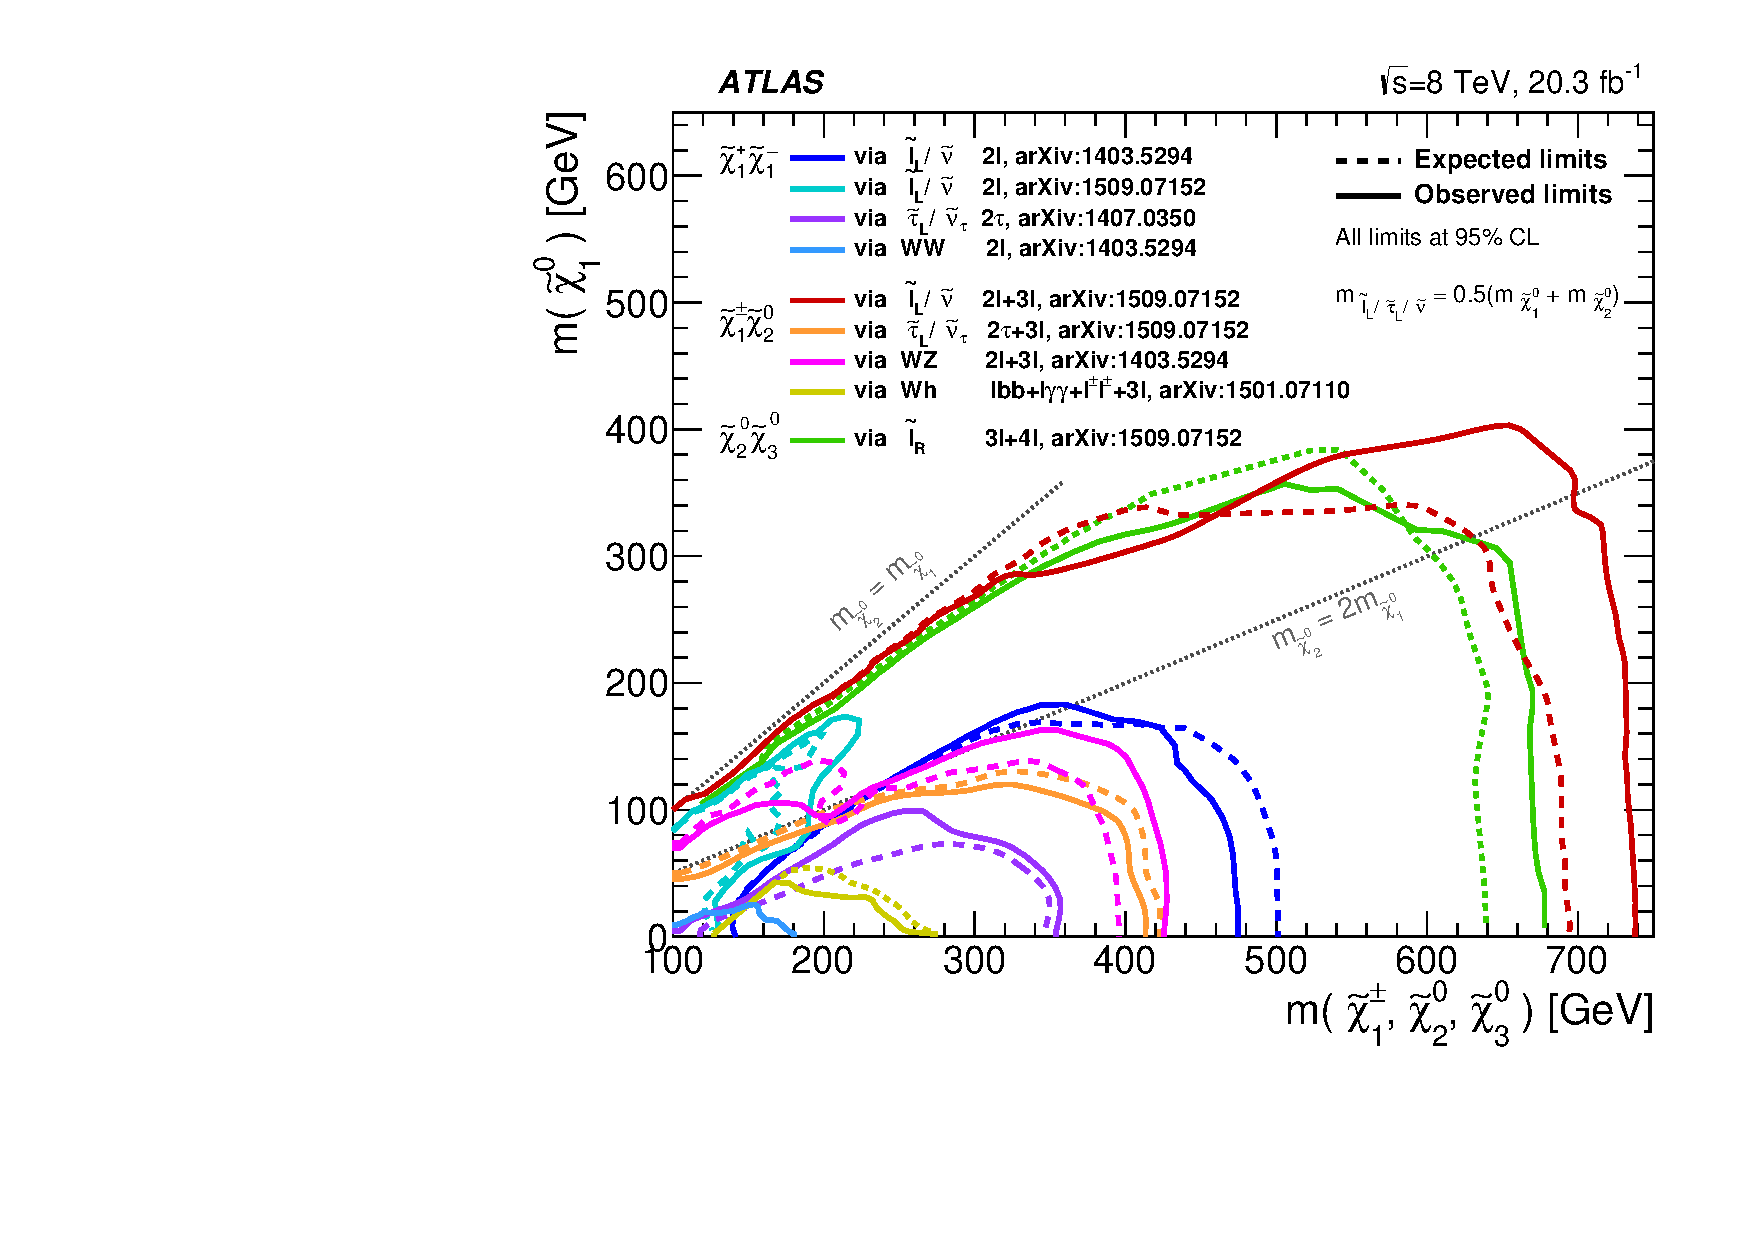
\includegraphics[width=0.7\textwidth]{ATLAS_SUSY_EWSummary}
  \caption{Run 1 summary.}
  \label{fig_run1_ew_results}
\end{figure}

Figure~\ref{fig_run1_soft3l_ss2l} shows the sensitivity of soft/ISR $3l$ and same-sign $2l$ selection. In the left, only $3l$ soft/ISR selection is given separately becasue the contribution from same-sign $2l$ is quite poor (Fig.~\ref{fig_run1_sen1}c). However, as shown in the right figure, the same-sign $2l$ is more sensitive the the case $m_{\susy{l}}=0.95m_{\chinoonepm}+0.5m_{\ninoone}$. The separate limits for the later case is shown in Fig.~\ref{fig_run1_sen2}.
\begin{figure}
  \centering
  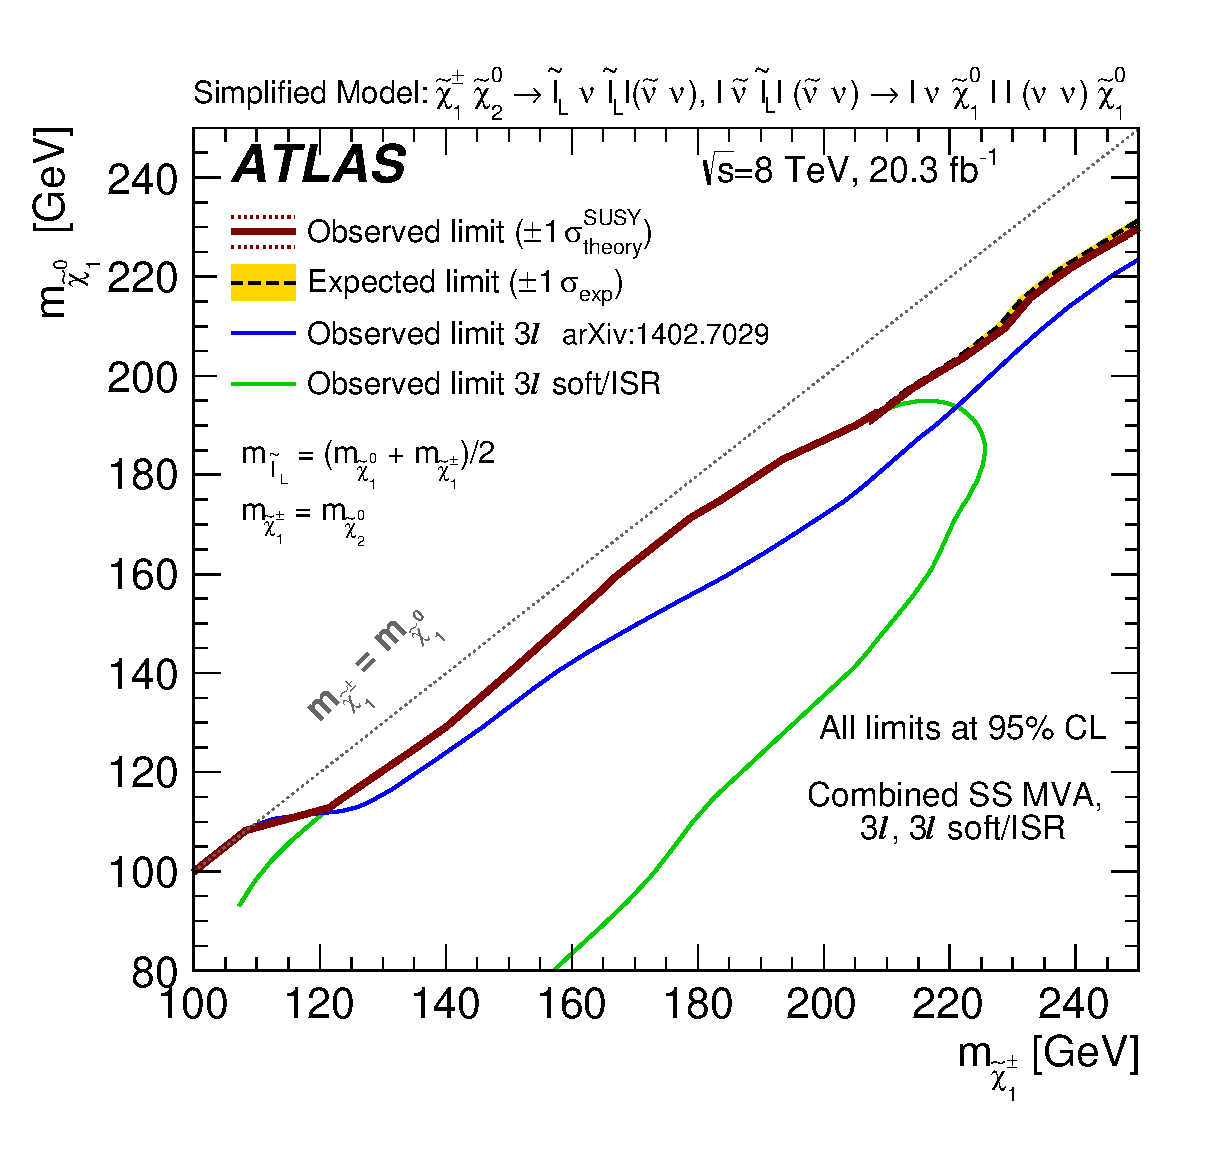
\includegraphics[width=0.49\textwidth]{SUSY_2014_05/fig_17a}
  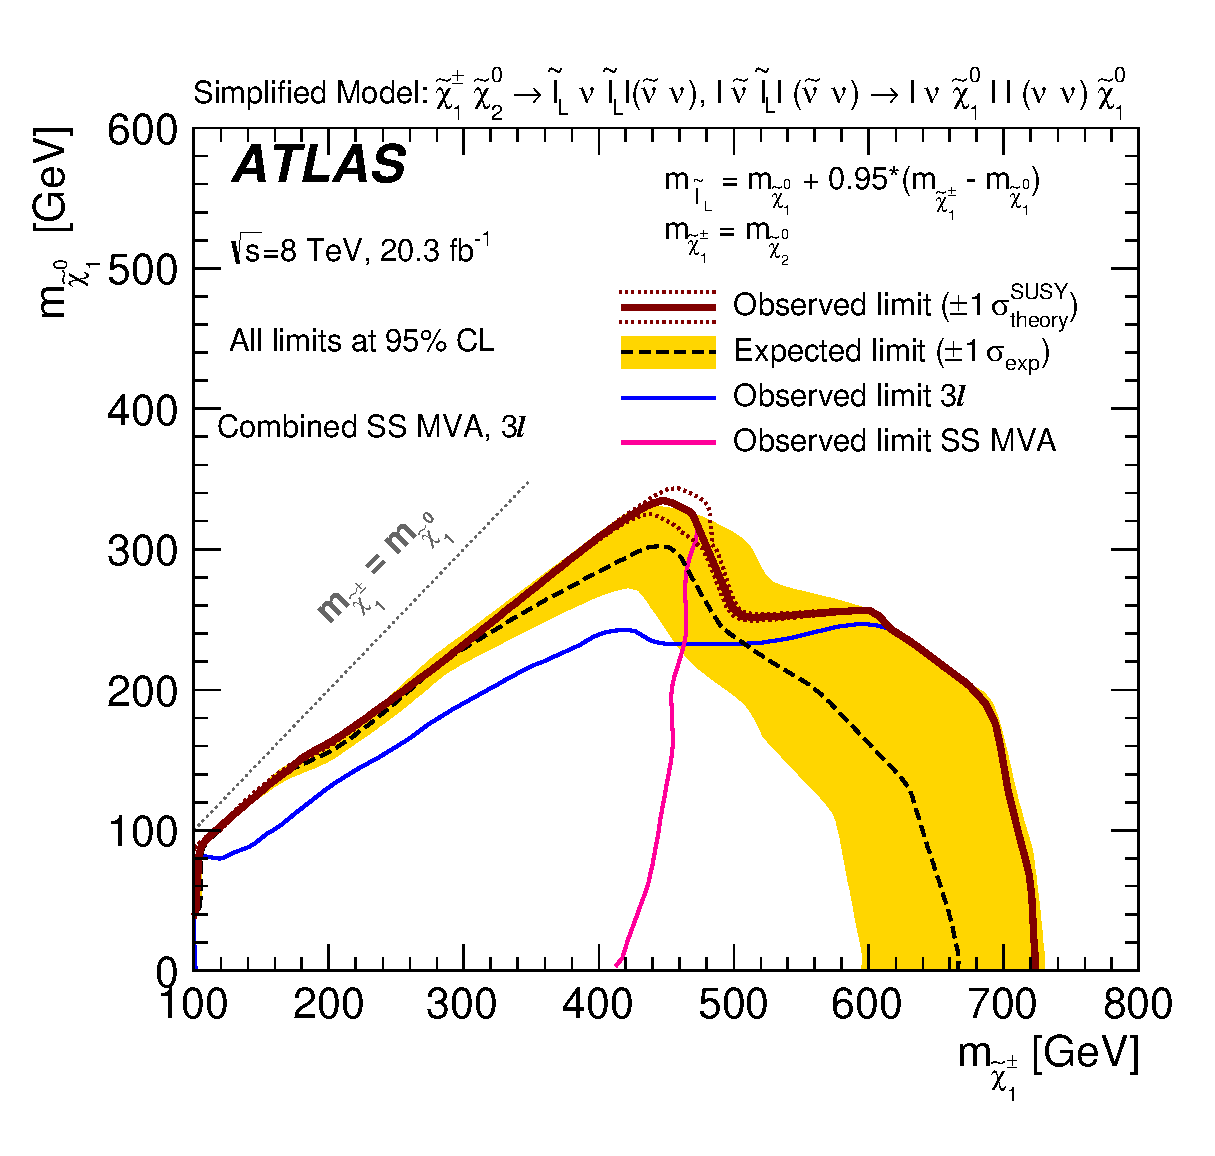
\includegraphics[width=0.49\textwidth]{SUSY_2014_05/fig_17b}
  \caption{The sensitive region of $3l$ soft/ISR selection comparing/combining with the old $3l$ selection (left). The sensitivity of $3l$ soft/ISR selection and same-sign $2l$ is also compared/combined (right). Taken from Ref.~\cite{Aad:2015eda}.}
  \label{fig_run1_soft3l_ss2l}
\end{figure}


% The sensitivity of SS selection is not good in the half mass senario (Fig.~\ref{fig_run1_sen1}), but has strong sensitivity in viarable mass senario (Fig.~\ref{fig_run1_sen2}).

\begin{figure}
  \centering
  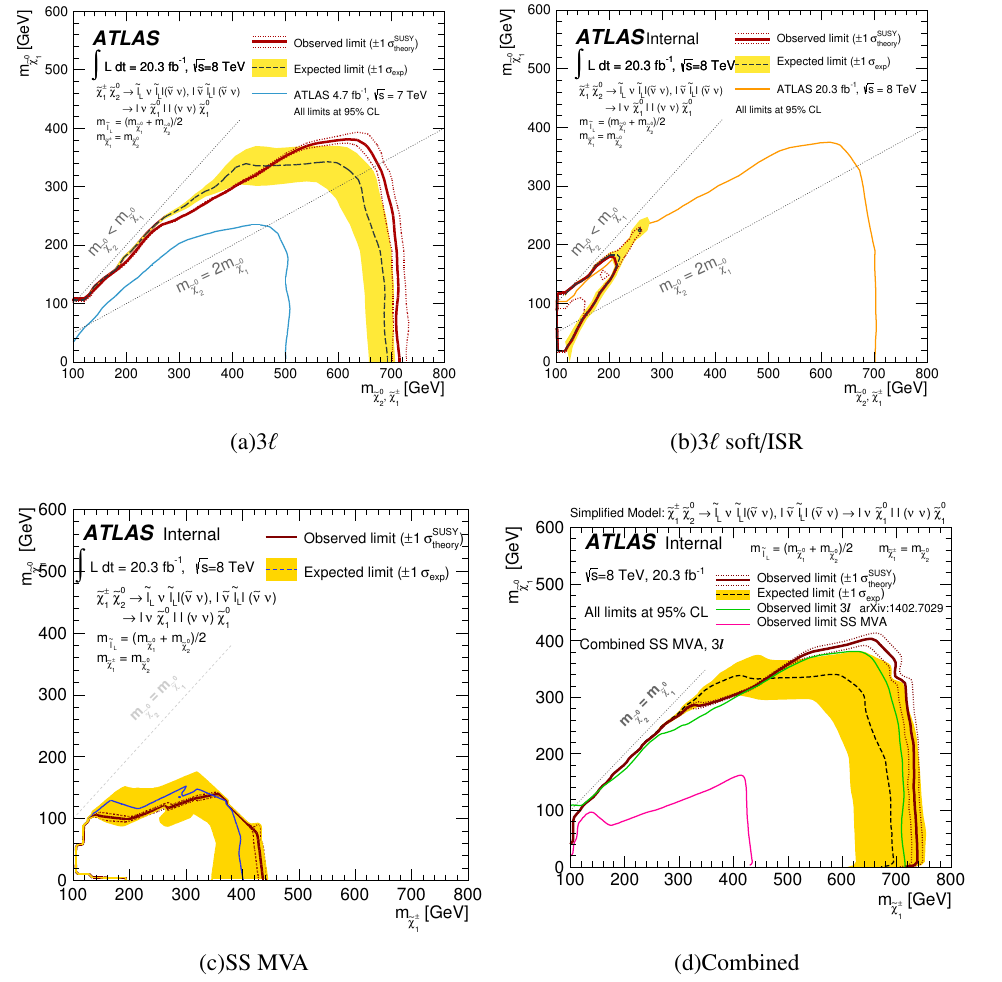
\includegraphics[width=0.9\textwidth]{ATL_COM_PHYS_2015_011/fig_7}
  \caption{Figure 7 of Ref.~\cite{Grout:1981548}}
\label{fig_run1_sen1}
\end{figure}

\begin{figure}
  \centering
  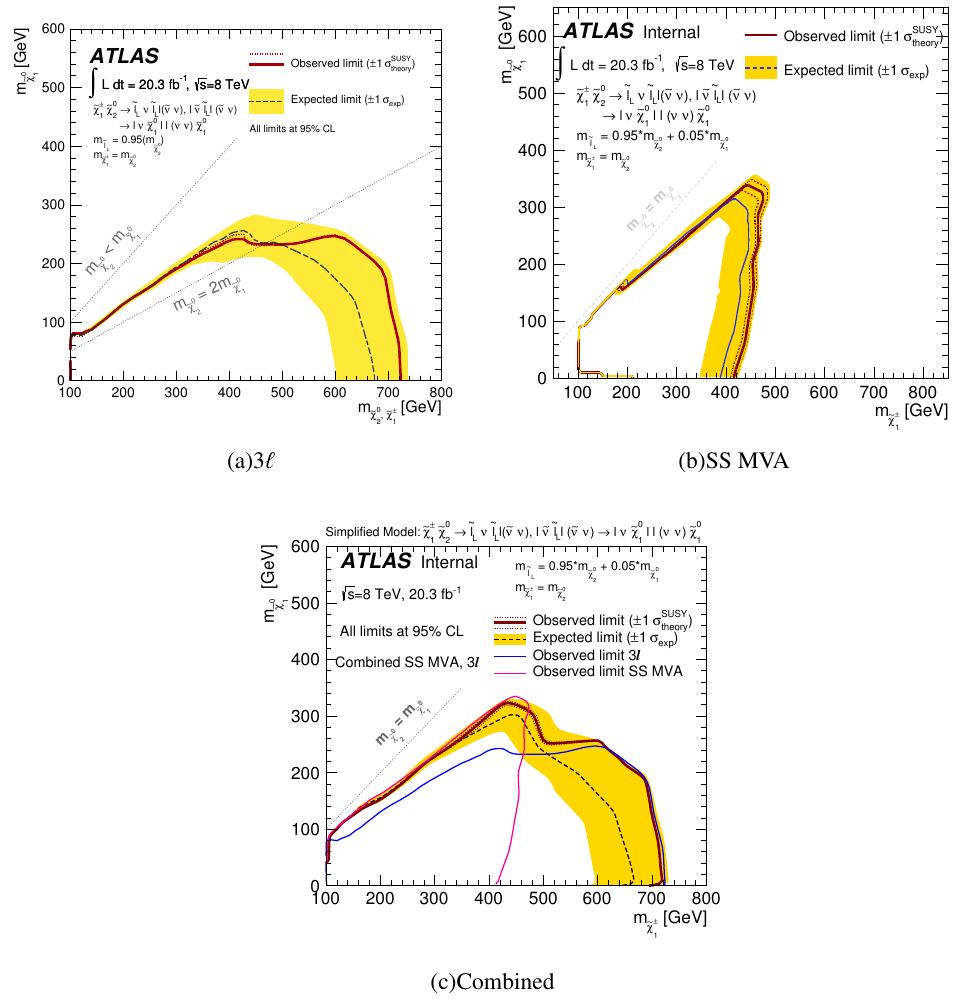
\includegraphics[width=0.9\textwidth]{ATL_COM_PHYS_2015_011/fig_8}
  \caption{Figure 8 of Ref.~\cite{Grout:1981548}}
\label{fig_run1_sen2}
\end{figure}


% \begin{figure}
%   \centering
%   \includegraphics[width=0.49\textwidth]{SUSY_2014_05/fig_19a}
%   \includegraphics[width=0.49\textwidth]{SUSY_2014_05/fig_19b}
% \end{figure}


The cross section of the signal is shown in Fig.~\ref{fig_sig_xsec}.
\begin{figure}
  \centering
  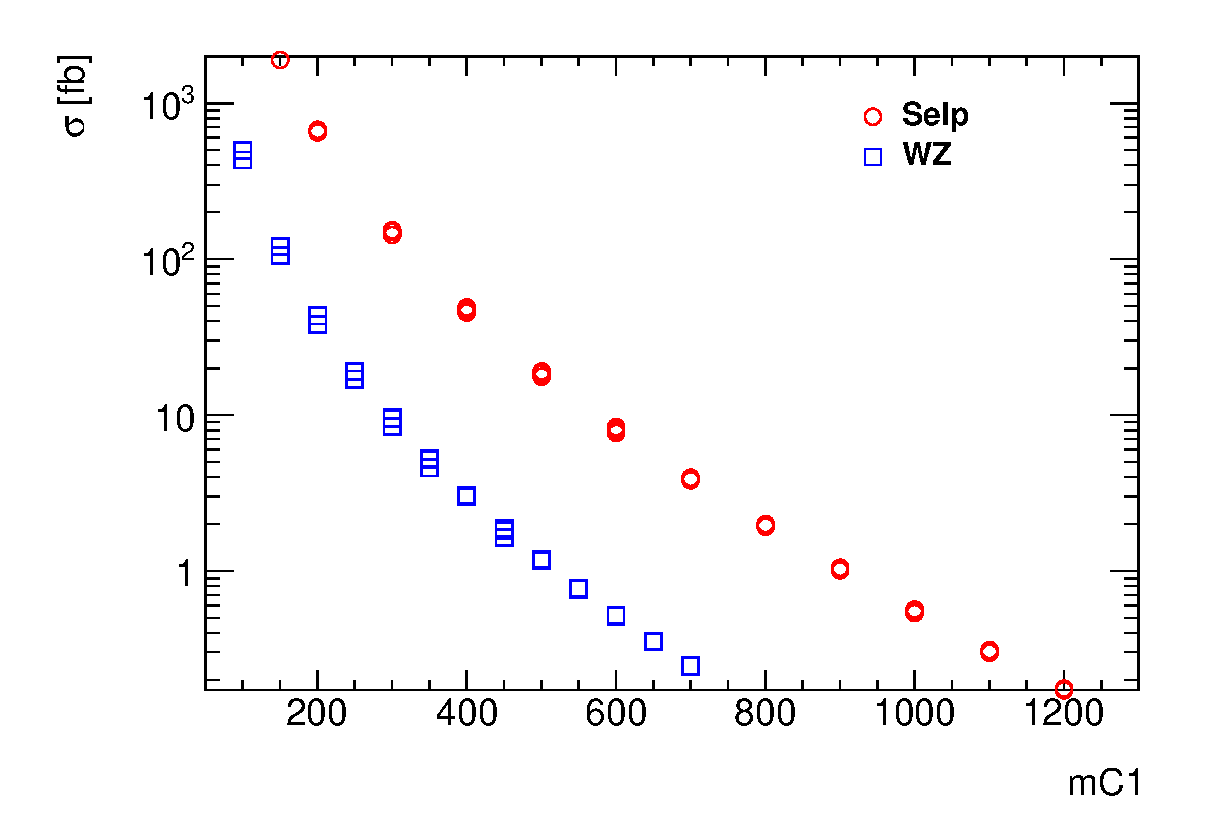
\includegraphics[width=0.49\textwidth]{sig_xSec}
  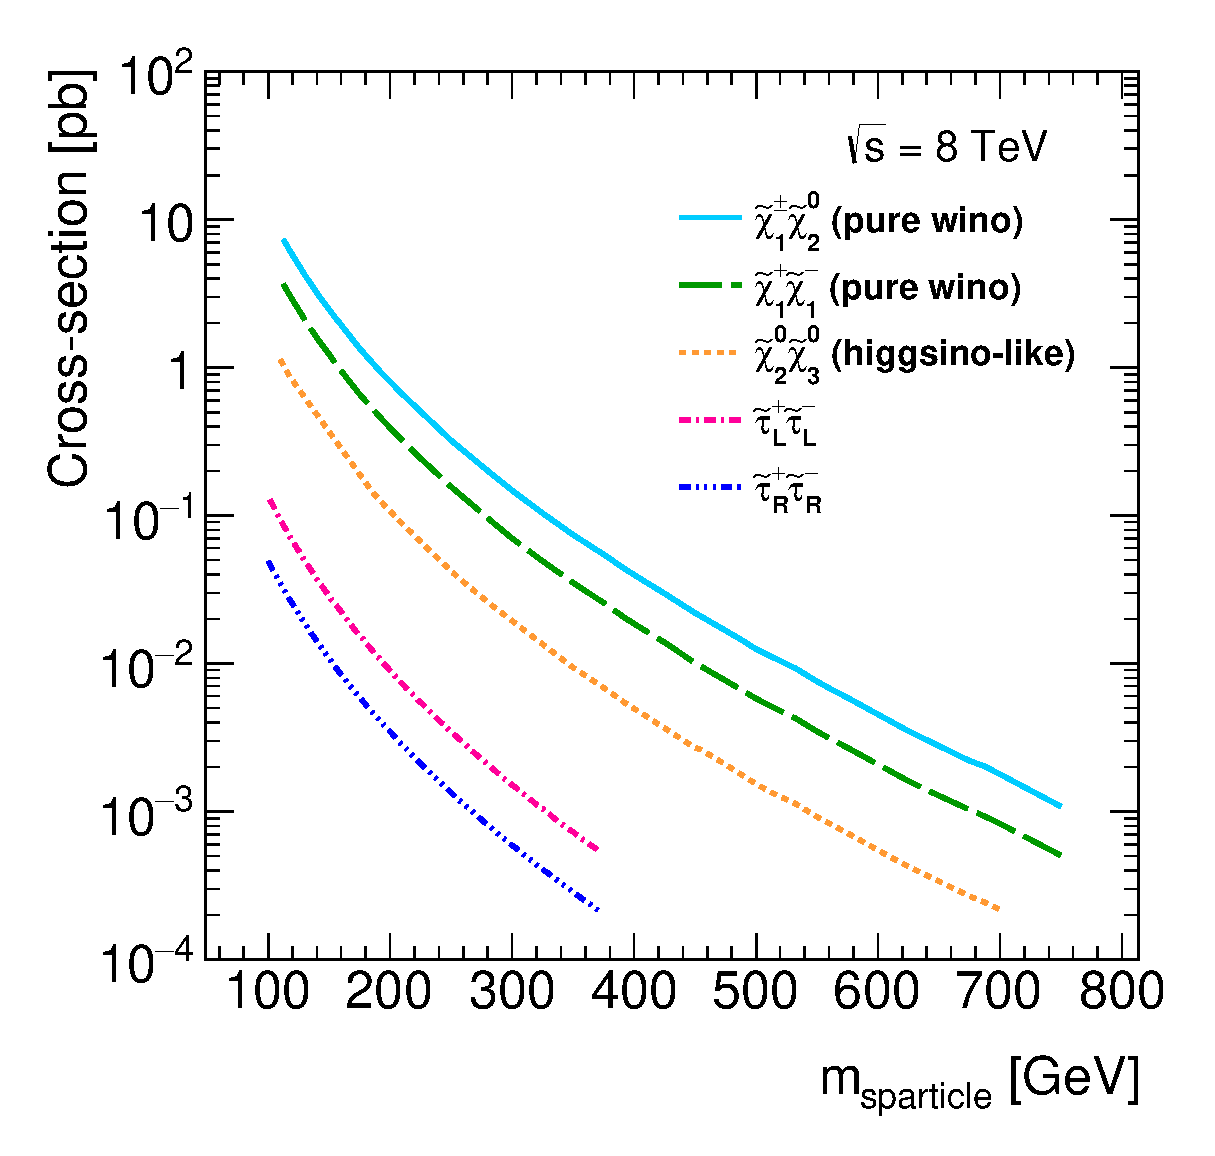
\includegraphics[width=0.49\textwidth]{SUSY_2014_05/fig_01}
  \caption{Cross section of $\chinoonepm\ninotwo$ production in $13\TeV$ and $8\TeV$ (from~\cite{Aad:2015eda}).}
  \label{fig_sig_xsec}
\end{figure}

%-------------------------------------------------------------------------------

\clearpage
%-------------------------------------------------------------------------------
\section{Samples}
\label{sec:samples}
 \subsection{Signal Sample Grid}
\begin{figure}
  \centering
  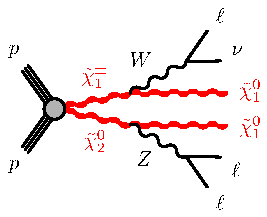
\includegraphics[width=0.35\textwidth]{C1N2-lllvN1N1-WZ}
  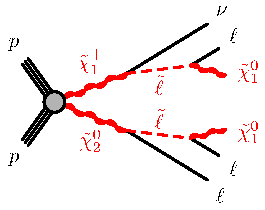
\includegraphics[width=0.35\textwidth]{C1N2-lllvN1N1-slsl}
  \caption{Deacy vis $\susy{l}$.}
  \label{fig_grid_sl}
\end{figure}
Grid infomation from $3l$ walkthrough note.
\begin{figure}
  \centering
  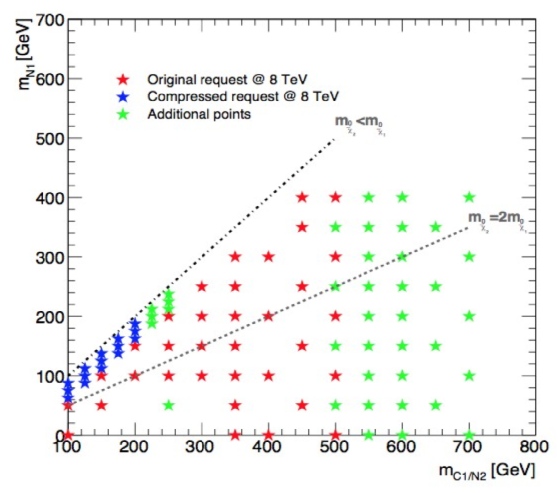
\includegraphics[width=0.49\textwidth]{C1N2_viaWZ3L_13TeC_newDesign}
  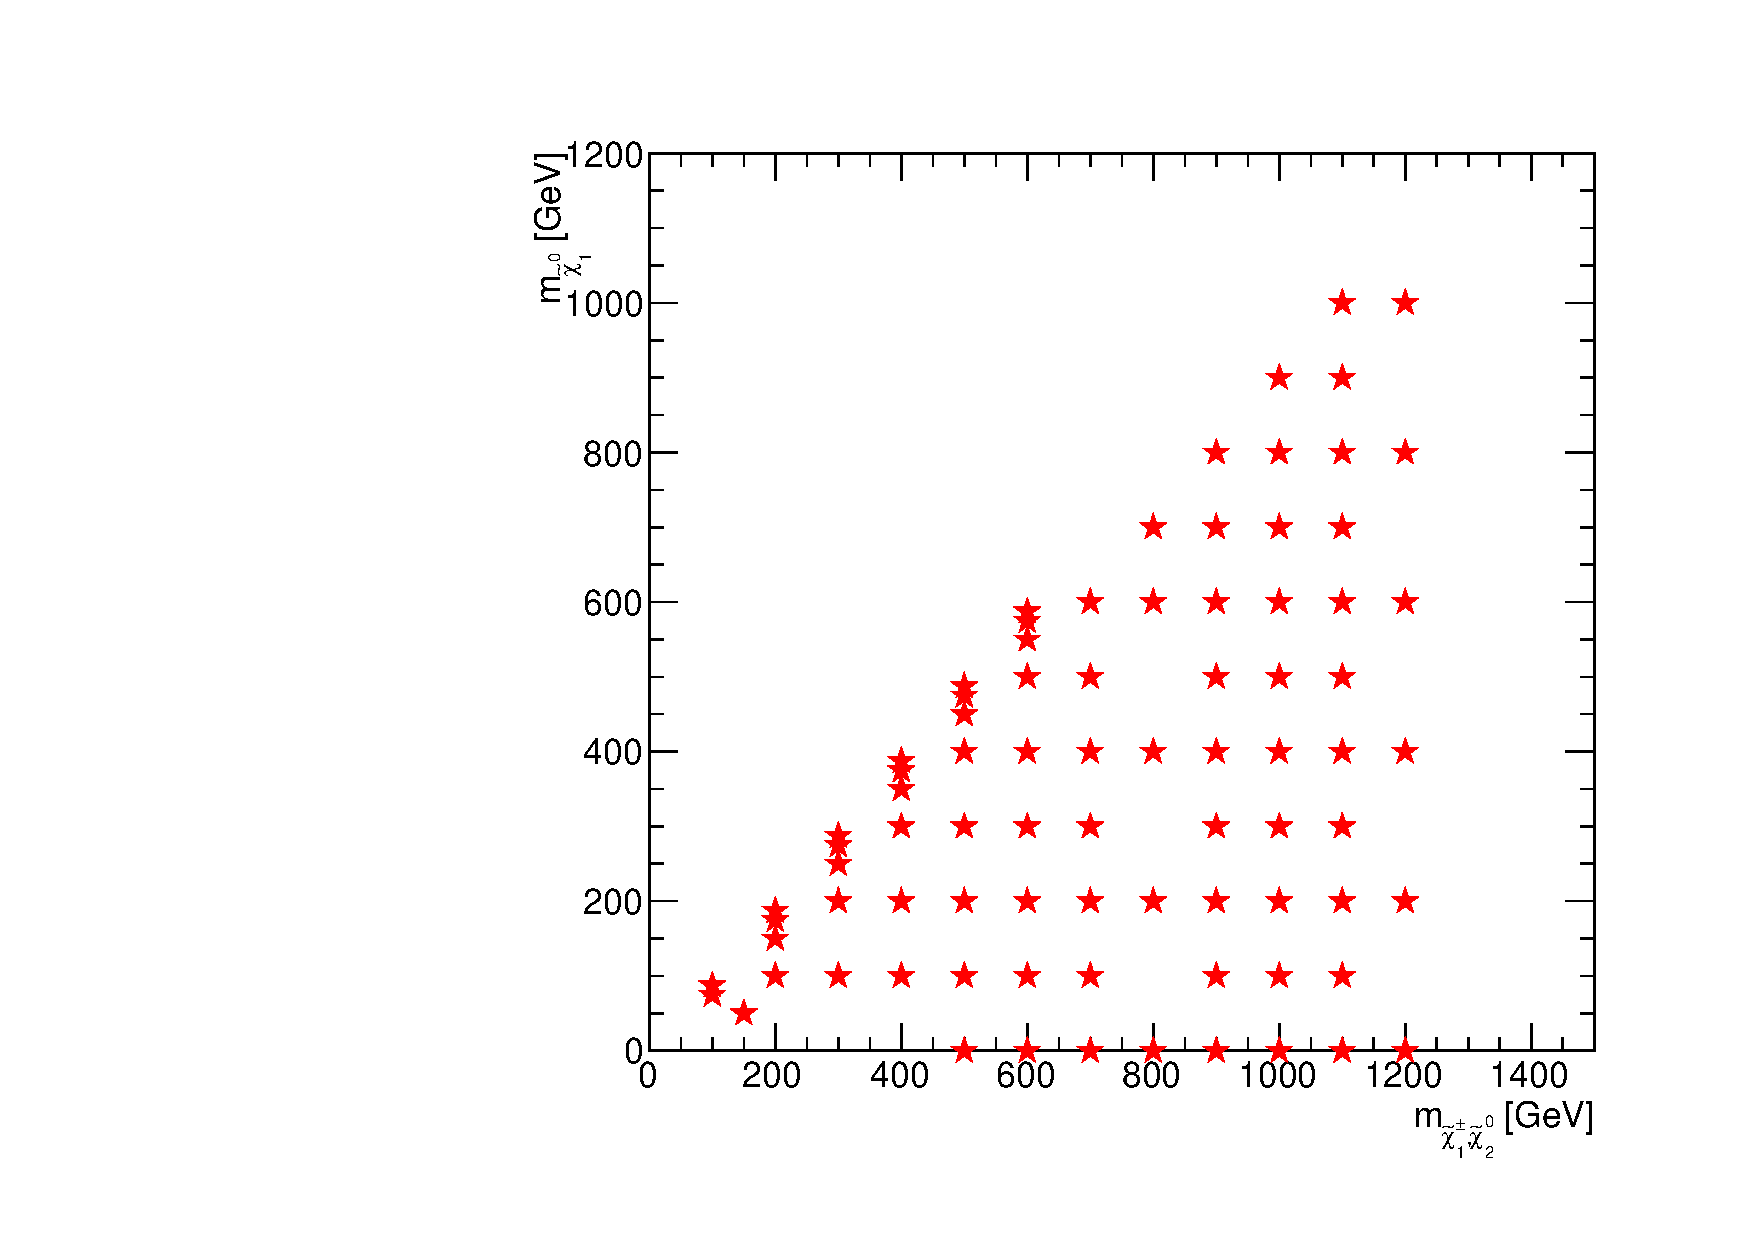
\includegraphics[width=0.49\textwidth]{C1N2_viaSL_13TeC_newDesign}
  \caption{Deacy vis $\susy{l}$.}
  \label{fig_grid_sl}
\end{figure}


The sample for $x=0.95$ mass splitting need to be requested.

\subsection{Background Simulation}
The description of the background MC.

%-------------------------------------------------------------------------------

\clearpage
%-------------------------------------------------------------------------------
\section{Event Selection}
\label{sec:selection}
\subsection{Object Definition}
The definition of all objects goes here.

\subsubsection{Electron}
The electron passing following selections are called ``Baseline electron'';
\begin{itemize}
  \item $\pt>10\GeV$, $|\eta|<2.47$
  \item \verb+LooseAndBLayerLLH+ ID
\end{itemize}

The baseline electron is considered as ``Signal electron'' if it furthermore satisfy following requirements:
\begin{itemize}
  \item \verb+TightLH+ ID
  \item $|d_0/\sigma(d_0)|<5$, $|z_0/\sigma(z_0)|<0.5$
  \item \verb+GradientLoose+ isolation
\end{itemize}

\subsubsection{Muon}
The baseline muon is defined as
\begin{itemize}
  \item $\pt>10\GeV$, $|\eta|<2.7$
\end{itemize}

Signal muon is defined as
\begin{itemize}
  \item \verb+Medium+ ID
  \item $|d_0/\sigma(d_0)|<3$, $|z_0/\sigma(z_0)|<0.5$
  \item \verb+GradientLoose+ isolation
  \item Cosmic mouon veto: $z_0<1$~mm, $d_0<0.2$~mm
  \item Bad muon veto: $\sigma(q/p)/(q/p)<0.2$
\end{itemize}

\subsubsection{Photon}

\subsubsection{$\tau$ lepton}
In the signal sample, $\tau$ final states are also included. Probalby we also need to select $\tau$ for
\begin{enumerate}
  \item $\tau$ veto
  \item Overlap removal
\end{enumerate}


\subsubsection{Jet}
\begin{itemize}
  \item \verb+EMTopo+ Jets
  \item $\pt>20\GeV$, $|\eta|<2.8$
  \item \verb+JVT+$>0.64$ for jets with $|\eta|<2.4$
  \item Bad jet veto for $\pt<50\GeV$ jets: not \verb+LooseBad+, not pileup jet (\verb+JVT+$<0.64$, $|\eta|<2.4$, $\pt<50\GeV$)
\end{itemize}

{\bf Central jets}

{\bf $b$-jets}


\subsection{Signal Regions}
\subsubsection{Useful Variables}
{\bf Missing transverse energy: $\met$}\\
$\met$ is calculated using baseline objects together with \verb+SoftTerms+.

{\bf Transverse mass: $\mT2$}\\
Defintion of $\mT2$


\subsubsection{SR definitions}

The definition of signal regions and their optimization goes here.

\begin{itemize}
  \item Trigger requirement
  \item Multiplicity of the objects
  \item Other variables
\end{itemize}

The optimization of the SR is given in Appendix.
% \subsubsection{Control Regions}
% 
% \subsubsection{Validtion Regions}

%-------------------------------------------------------------------------------

\clearpage
%-------------------------------------------------------------------------------
\section{Background}
\label{sec:bkg}
\subsection{Electro-weak Background}
The background from diboson processes.
\begin{itemize}
  \item Cross section and $k$-factors
  \item Pileup reweighting
  \item Efficinecy scale factors
  \item Conrol region and validation region
\end{itemize}

\subsection{Jet mis-identified as leptons}
The fake rate measurement and fake background estimation goes here.
Using control sample together with the fake rate.

\subsection{Lepton charge mis-identification}

\subsubsection*{Mechanisms}
The misidentification rate of leptons is governed by \\
\begin{align}
-\langle\frac{dE}{dx}\rangle \varpropto \frac{E}{m^2}
\end{align}
Thus this rate is significant for electrons and high energy ($E > 400GeV$) muons. Therefore only the electron charge misidentification is calculated. \\

Electron charge misidentification is due to:
\begin{enumerate}
\item Bremsstrahlung photon and conversion electron
\item Track misidentification
\end{enumerate}

Since a magnetic field exists within the detector, it is possible to infer the charge and momentum of electrons by the curvature of their tracks. However, there are cases when the reconstruction gives the wrong charge. 

\begin{figure}[h]
\centering
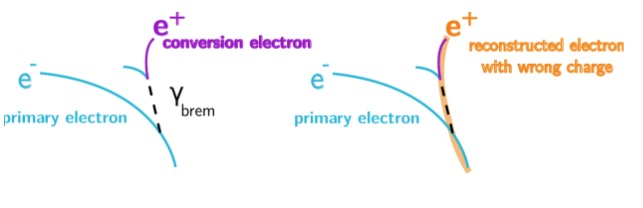
\includegraphics[width=\textwidth]{ChargeMisID/Brem}
\caption[Electron charge misidentification by bremsstrahlung]{Bremsstrahlung}
\label{fig:brem}
\end{figure}
\begin{figure}[h]
\centering
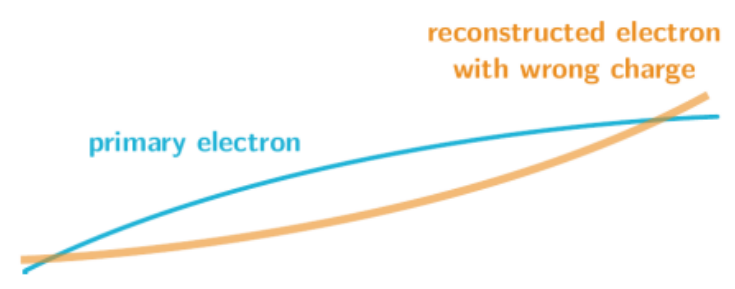
\includegraphics[width=\textwidth]{ChargeMisID/WrongTrack}
\caption[Electron charge misidentification by track mis-reconstruction]{Track mis-reconstruction}
\label{fig:wrong-track}
\end{figure}

\underline{Bremsstrahlung} \\
Charge misidentification may occur when an electron radiates a photon early in the detector (in the beampipe, or the first layers of the inner tracker). The radiated photon may then undergo pair production, and the converted electrons would leave tracks in the inner tracker.  One of these wrong tracks may then be matched to an energy deposit inside the calorimeter. In case the electron that left the track has the opposite charge to the original, then the charge inferred would be opposite to the charge of the original electron \cite{ElectronReco2011}. (Figure \ref{fig:brem}). 

The probability of bremsstrahlung increases with the amount of material the electron interacts with. Hence as the material budget of the detector changes with $|\eta|$ (Figure \ref{fig:material-budget}), it is expected that the charge misidentification rate ought to depend on  $|\eta|$.

\begin{figure}[h]
\centering
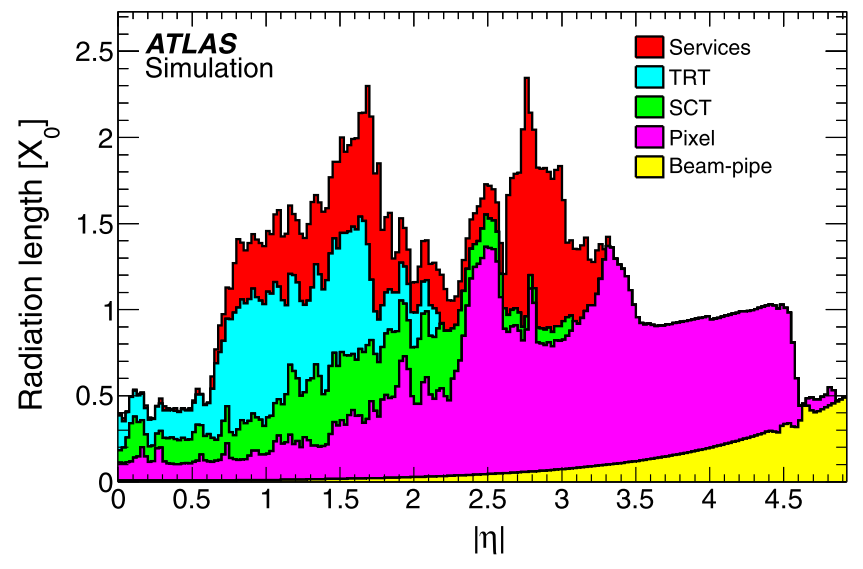
\includegraphics[scale=0.4]{ChargeMisID/Material-budget.png}
\caption[Amount of material traversed by a particle as a function of $|\eta|$]{Amount of material in front of the solenoid magnet and EM calorimeters traversed by a particle as a function of $|\eta|$. Figure from \cite{ElectronReco2011}.}
\label{fig:material-budget}
\end{figure}

\underline{Track mis-reconstruction}\\
Another possible source of charge misidentification is track mis-reconstruction. The near straight track of a high $p_T$ electron may be reconstructed with the opposite curvature, thus giving the opposite sign. (Figure \ref{fig:wrong-track})

\subsubsection*{Likelihood Method for Measuring Charge misID}
$Z\rightarrow e^\pm e^\mp$ events are studied for its relatively clean signal (see Figure \ref{fig:mll_ee_OS}) and because, by charge conservation,  the two daughter electrons of the $Z$ must be of opposite sign. In principle, if a $Z\rightarrow e^\pm e^\pm$ event is found, it must the case that the charge of one electron has been misidentified. The likelihood method was used to measure the charge misidentification rate. An alternative method, the tag-and-probe method, was also attempted; the results obtained were unsatisfactory. 

\begin{figure}[h]
\centering
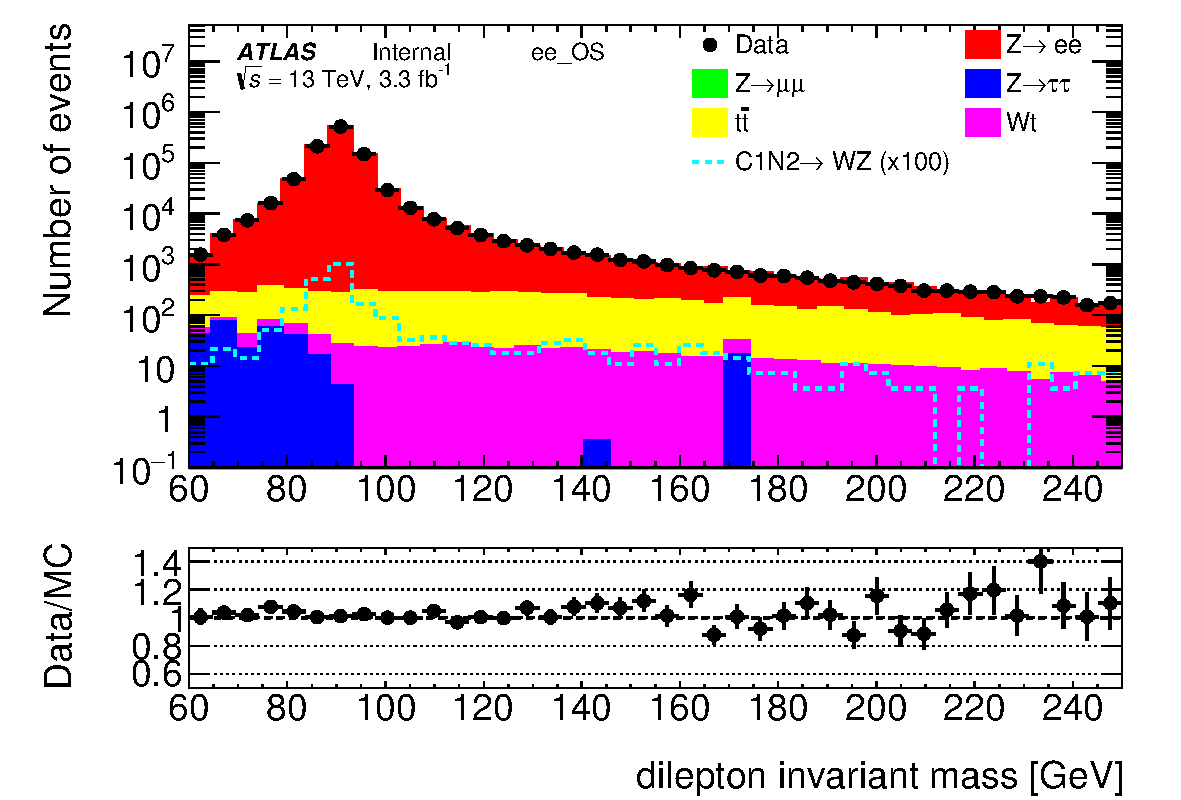
\includegraphics[scale=0.6]{ChargeMisID/mll_ee_OS.pdf}
\caption[Distribution of opposite-sign dielectron events]{Distribution of opposite-sign dielectron events. Note that the region near the Z mass $(91.2\ GeV)$ the signal is dominated by $Z\rightarrow e^\pm e^\mp$ events by at least 2 orders of magnitude. Plot by Lo Cheuk Yee, HKU.}
\label{fig:mll_ee_OS}
\end{figure}

The most likely rate of charge misidentification is determined by extremizing a likelihood function. 

$Z\rightarrow ee$ events were selected by imposing the following cuts:
\begin{itemize}
\item Events with two electrons
\item $75\ GeV < m_{ee} < 100\ GeV$
\item $\Delta \phi > 2$
\item Both same-sign and opposite-sign events are selected
\end{itemize}

The probability of observing a same sign event is:
\begin{equation}
p = P(e_1 \text{ correct sign})P(e_2 \text{ wrong sign}) + P(e_1 \text{ wrong sign})P(e_2 \text{ correct sign})
\end{equation}

Each electron is assigned a bin which depends on its $\eta$ and $p_T$. For events where one electron falls into bin $i$ and the other electron falls into bin $j$, the probability of observing a same-sign event is: 
\begin{equation}
p =(1-\epsilon_i)\epsilon_j + (1-\epsilon_j)\epsilon_i
\end{equation}
where $\epsilon_i$ is the charge misidentification rate in bin $i$.

The expected number of same-sign events is given by
\begin{equation}
N^{exp}_{SS} = np 
\end{equation}

A binomial distribution of observing $nss$ same-sign events is expected:
\begin{equation}
P(nss |\epsilon_i, \epsilon_j) =  C^n_{nss} p^{nss}(1-p)^{n-nss}
\end{equation}

Since $p$ is small, this can be approximated well by a Poisson distribution: 
\begin{equation}
P(nss |\epsilon_i, \epsilon_j) = \frac{(N^{exp}_{SS})^{nss} e^{-N^{exp}_{SS}}}{nss!}
\end{equation}

With this equation of the probability of observing $nss$ same-sign events given $\epsilon_i$ and $\epsilon_j$, the likelihood function of having $\epsilon_i$, $\epsilon_j$ given $nss$ observed same-sign events can be defined: 
\begin{equation}
L(\epsilon_i, \epsilon_j | nss) \equiv P(nss |\epsilon_i, \epsilon_j)
\end{equation}

For the likelihood across all combinations of bins $i,j$,
\begin{equation}
\mathcal{L} = \prod\nolimits_{i,j} L(\epsilon_i, \epsilon_j)
\end{equation}

By maxmizing the likelihood function, the most probable $\epsilon_i$, $\epsilon_j$ can be found for a given $nss$ observed same sign events. To simplify calculation, the logarithm function is applied to $\mathcal{L}$. To take advantage of the minimizer in ROOT, the negative of the function is minimized. 

The final function to be minimized is 

\begin{equation}
-\ln \mathcal{L} = -\sum\nolimits_{i,j} \Big\{ {nss}_{ij} \ln\big(n_{ij}[\epsilon_j(1-\epsilon_i) + \epsilon_i(1-\epsilon_j)]\big) - n_{ij}[\epsilon_j(1-\epsilon_i) + \epsilon_i(1-\epsilon_j)] - \ln (nss_{ij}!) \Big\}
\end{equation} 

\subsubsection*{Validation with Monte Carlo}
A Monte Carlo (MC) sample of simulated $Z \rightarrow ee$ events was used to develop and validate the likelihood algorithm. The information saved in the MC sample includes the \textit{truth} information of the simulated events, and the reconstructed event information produced from a detector simulator. 

%\footnote{MC sample used: \texttt{mc15\_13TeV:mc15\_13TeV.361106.PowhegPythia8EvtGen\_AZNLOCTEQ6L1\_Zee.merge.DAOD\_SUSY2.e3601\_s2576\_s2132\_r6765\_r6282\_p2419}} \todo{Fix this sample name. Should be included?}

For every reconstructed electron selected by the aforementioned conditions, an attempt was made to find the charge of the original daughter electron of Z. A reconstructed electron was first matched to a truth particle with the smallest $\Delta R = \sqrt{\Delta \phi^2 + \Delta \eta^2} < 0.1$ separation from the reconstructed electron. The truth particle was rejected if it was not an electron.\footnote{It could be the case that a hadron was misidentified as an electron \cite{ElectronReco2011}.} The decay path was then traversed upwards to find the original daughter electron of a Z boson. The truth particle was rejected if no Z boson was found in the path, or if the daughter particle of Z was not an electron.\footnote{It was found that sometimes the algorithm would match to a final-state radiation photon from Z.} An example of this algorithm is shown in Figure \ref{fig:find-daughter-electron}.

\begin{figure}[h!]
\centering
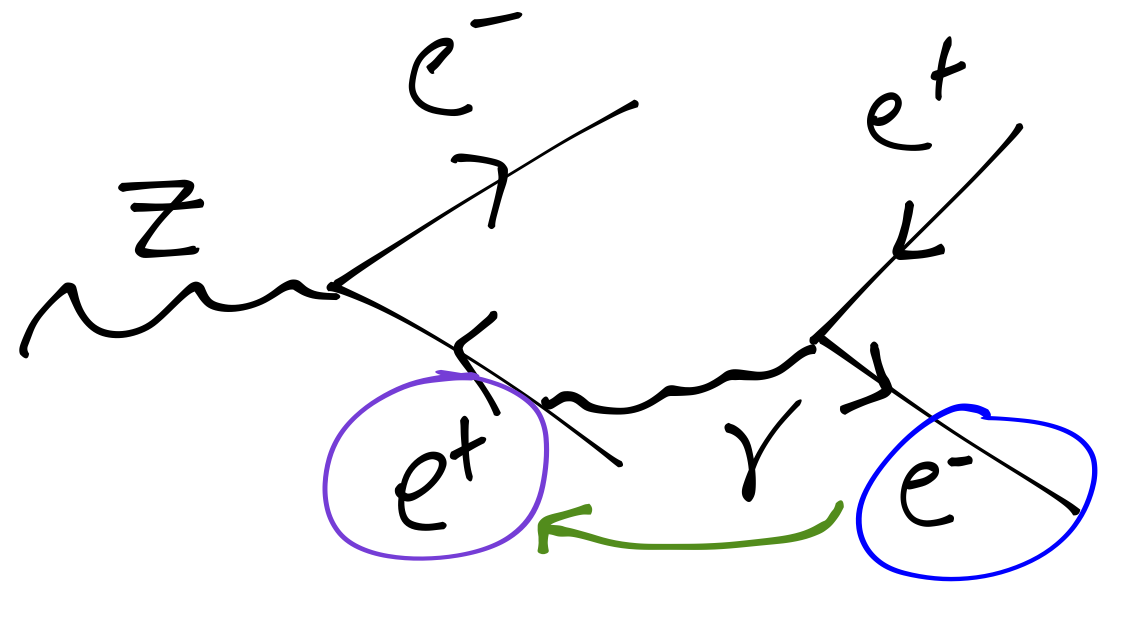
\includegraphics[scale=0.35]{ChargeMisID/MC-truth}
\caption[Finding the original daughter electron of Z]{Finding the  daughter electron of Z. The electron circled in blue is the truth electron matched to the reconstructed electron. The decay was traversed upwards to find the original daughter electron of a Z boson, circled in purple.}
\label{fig:find-daughter-electron}
\end{figure}

If the original electron daughter of Z was found, then it was considered to be the \textit{matched} electron of the reconstructed electron. If the charge of the matched electron was not identical to the charge of the reconstructed electron, then the charge was considered to be misidentified. Thus the true charge misidentification rate in each bin can be defined as:

\begin{equation}
\epsilon_{\text{MC}} = \frac{\text{Number of reconstructed electrons with charge opposite to its matched electron}}{\text{Total number of matched electrons}}
\end{equation}

\subsubsection*{Charge misID rates}
The charge misidentification rates of both LooseBaseline and Signal electrons were computed in bins of $|\eta|$ and $p_T$ (bin edges defined in Table \ref{table:binning}) by:
\begin{itemize}
\item the likelihood method on $3.2\  \text{fb}^{-1}$ of $pp$ collision data collected by ATLAS in 2015 (labeled in the plots as \textit{Data}),
\item the likelihood method on a $Z\rightarrow ee$ MC sample (labeled in the plots as \textit{MC LH}), and
\item extracting the true rates from the same MC sample (labeled in the plots as \textit{MC truth}).
\end{itemize}

\begin{table}[h!]
\centering
\begin{tabular}{c | c}
\textbf{Variable} & \textbf{Bin edges} \\
\hline
$|\eta|$ & 0, 0.5, 1, 1.37, 1.52, 1.8, 2.0, 2.5 \\
$p_T$ (GeV) &  20, 30, 40, 50, 60, 80, 120
\end{tabular}
\caption{Binning in $|\eta|$ and $p_T$}
\label{table:binning}
\end{table}

\begin{figure}[h!]
\centering
\subfloat[][Comparison of rates for LooseBaseline electrons]{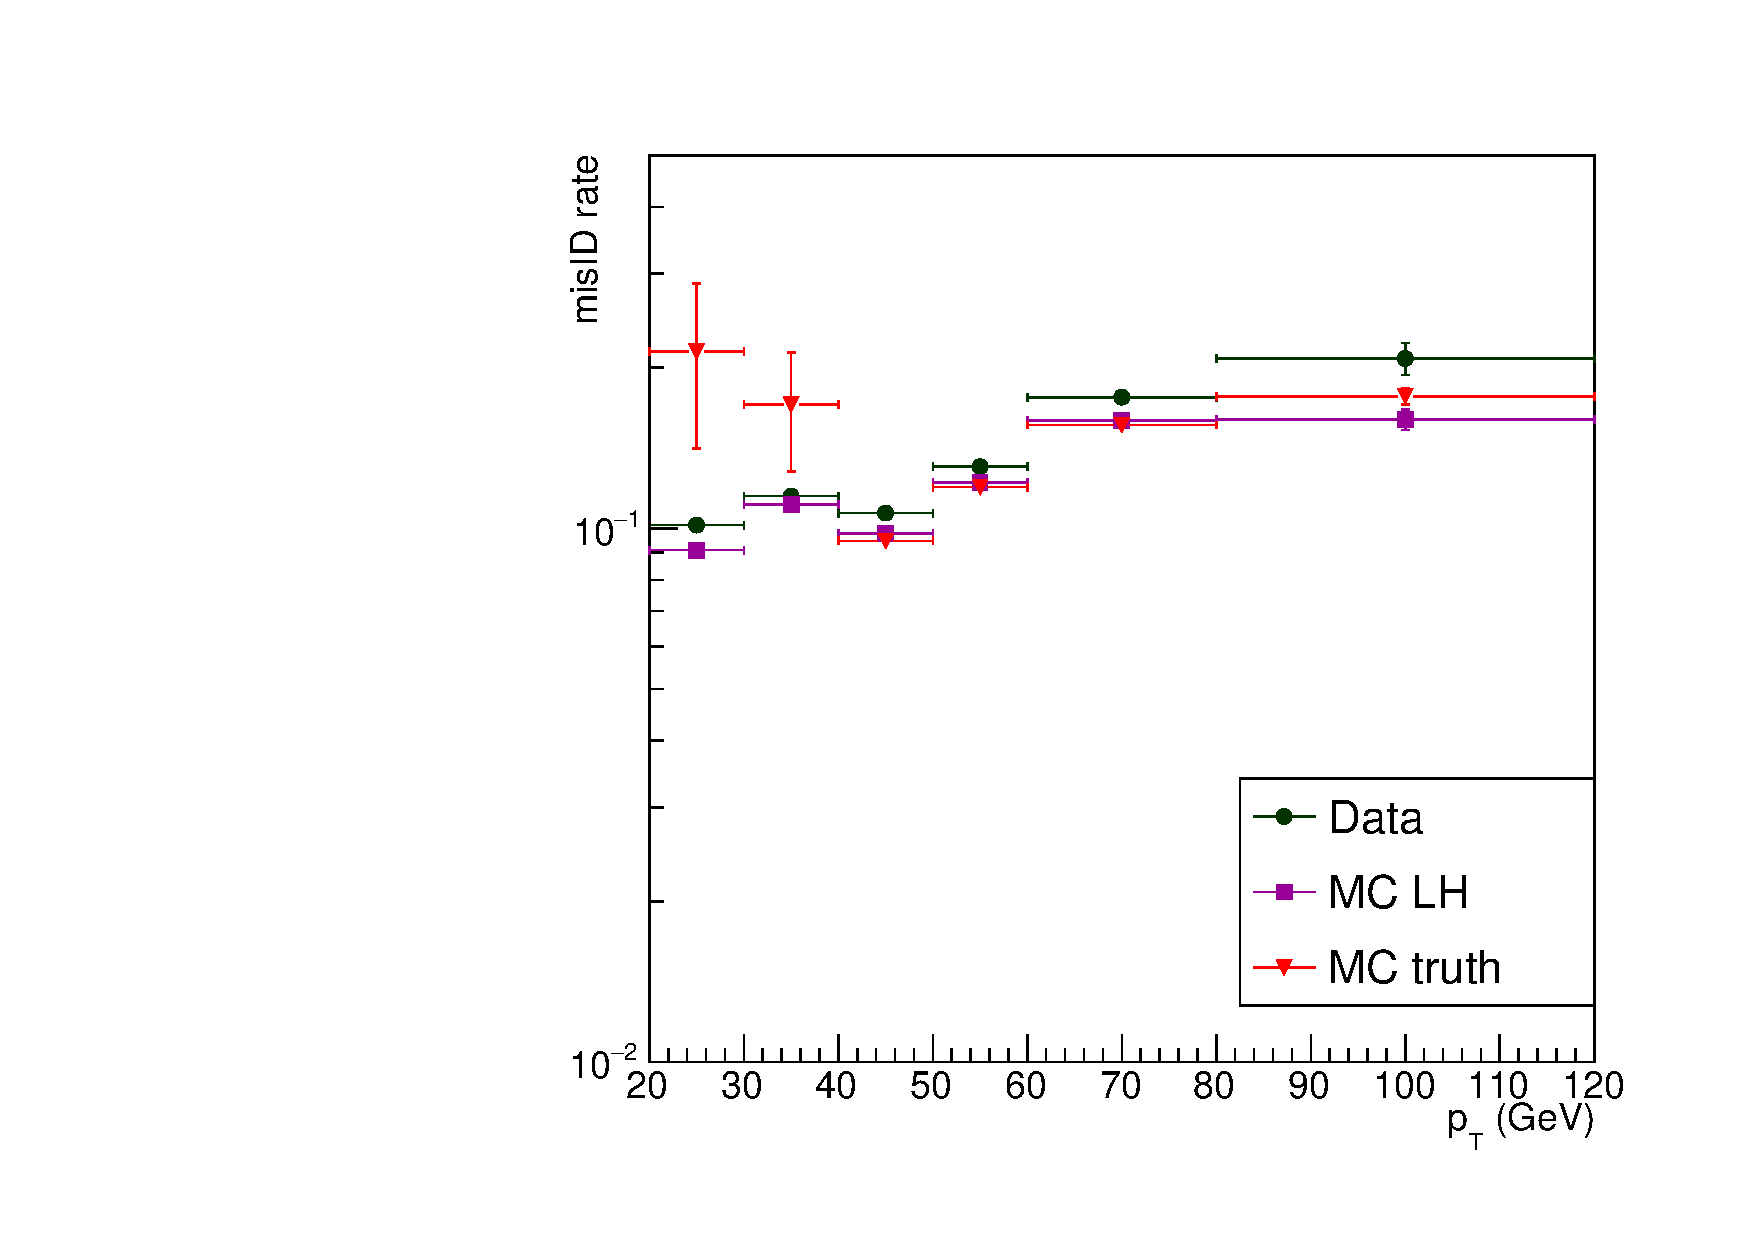
\includegraphics[scale=0.39]{ChargeMisID/WoSub_loose/Pt.pdf}}
\subfloat[][Comparison of rates for Signal electrons]{
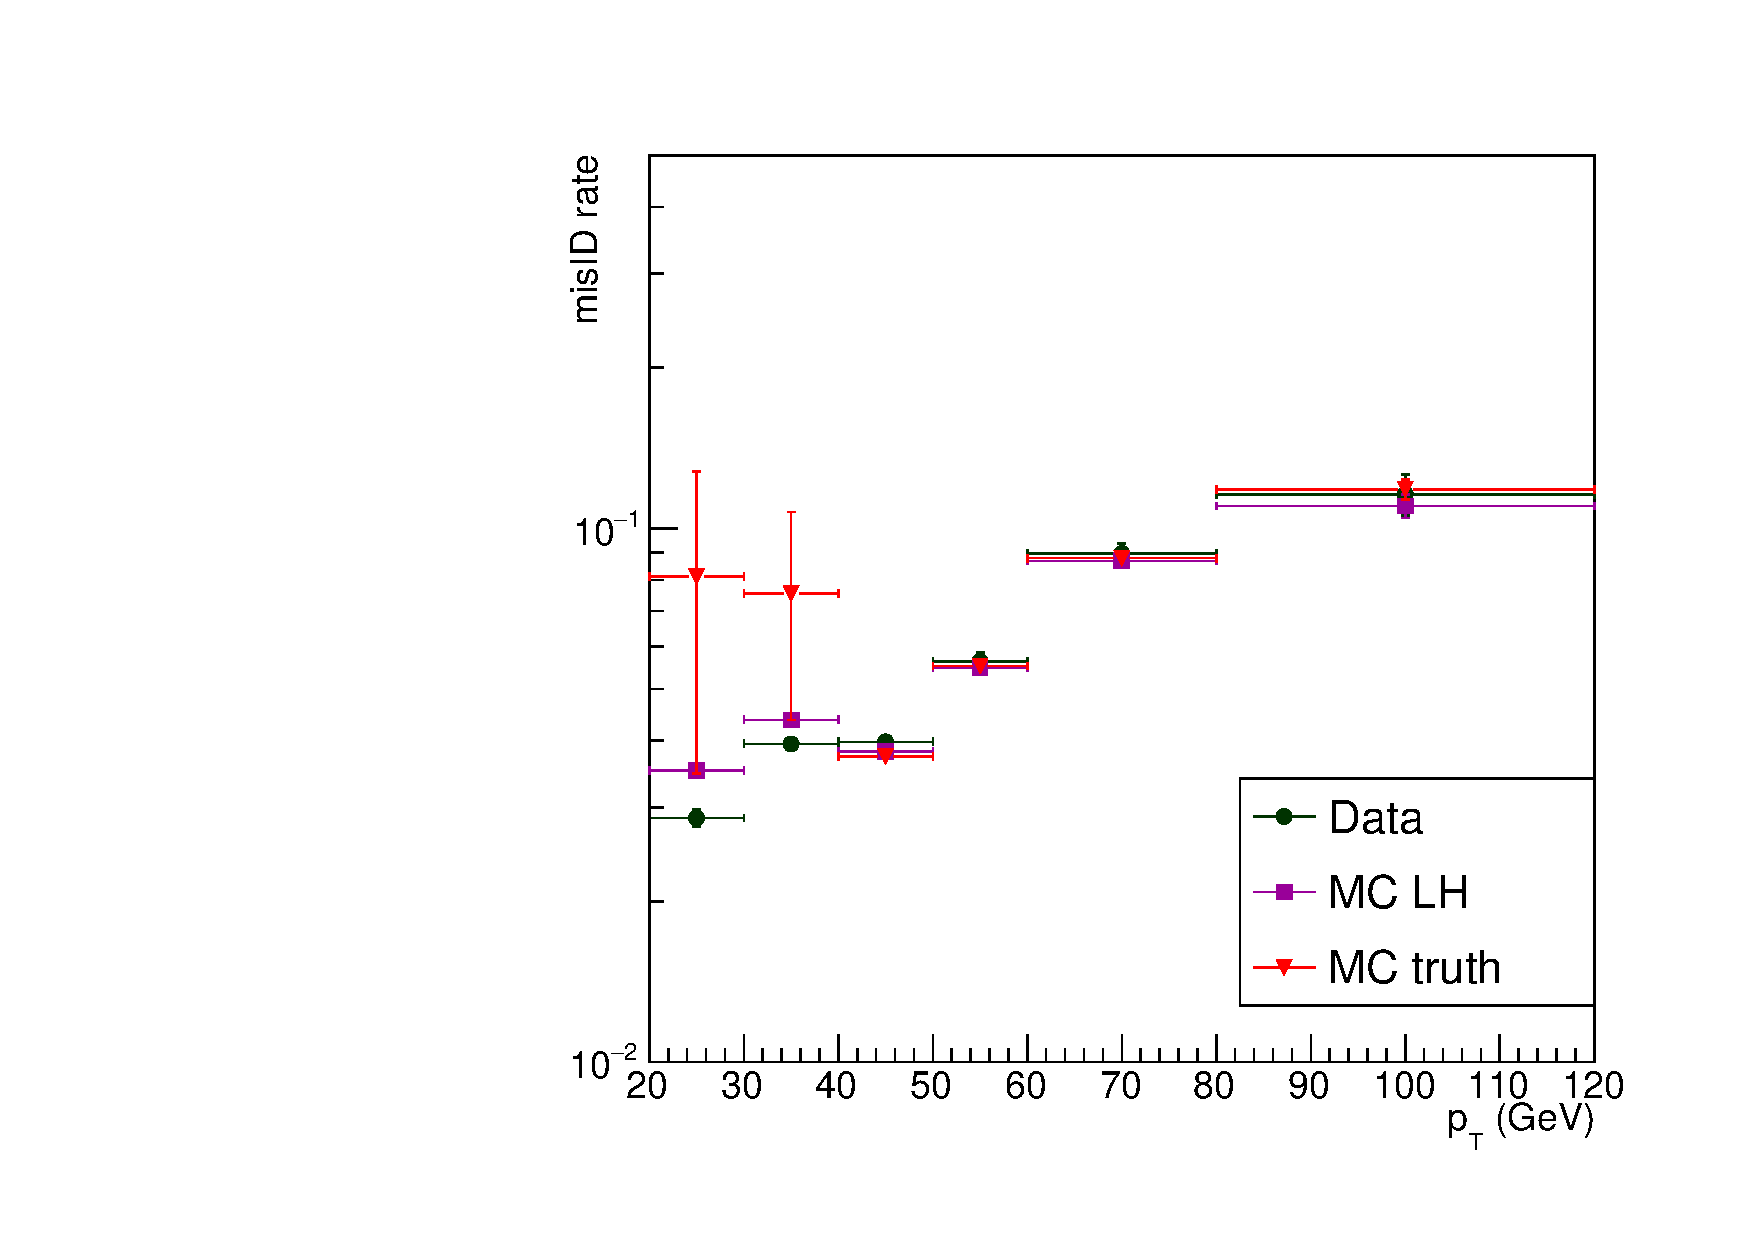
\includegraphics[scale=0.39]{ChargeMisID/WoSub_signal/Pt.pdf}}
\caption{Comparison of electron charge misidentification rates as a function of $p_T$}
\label{fig:rates-pt}
\end{figure}

\begin{figure}[h!]
\centering
\subfloat[][Comparison of rates for LooseBaseline electrons]{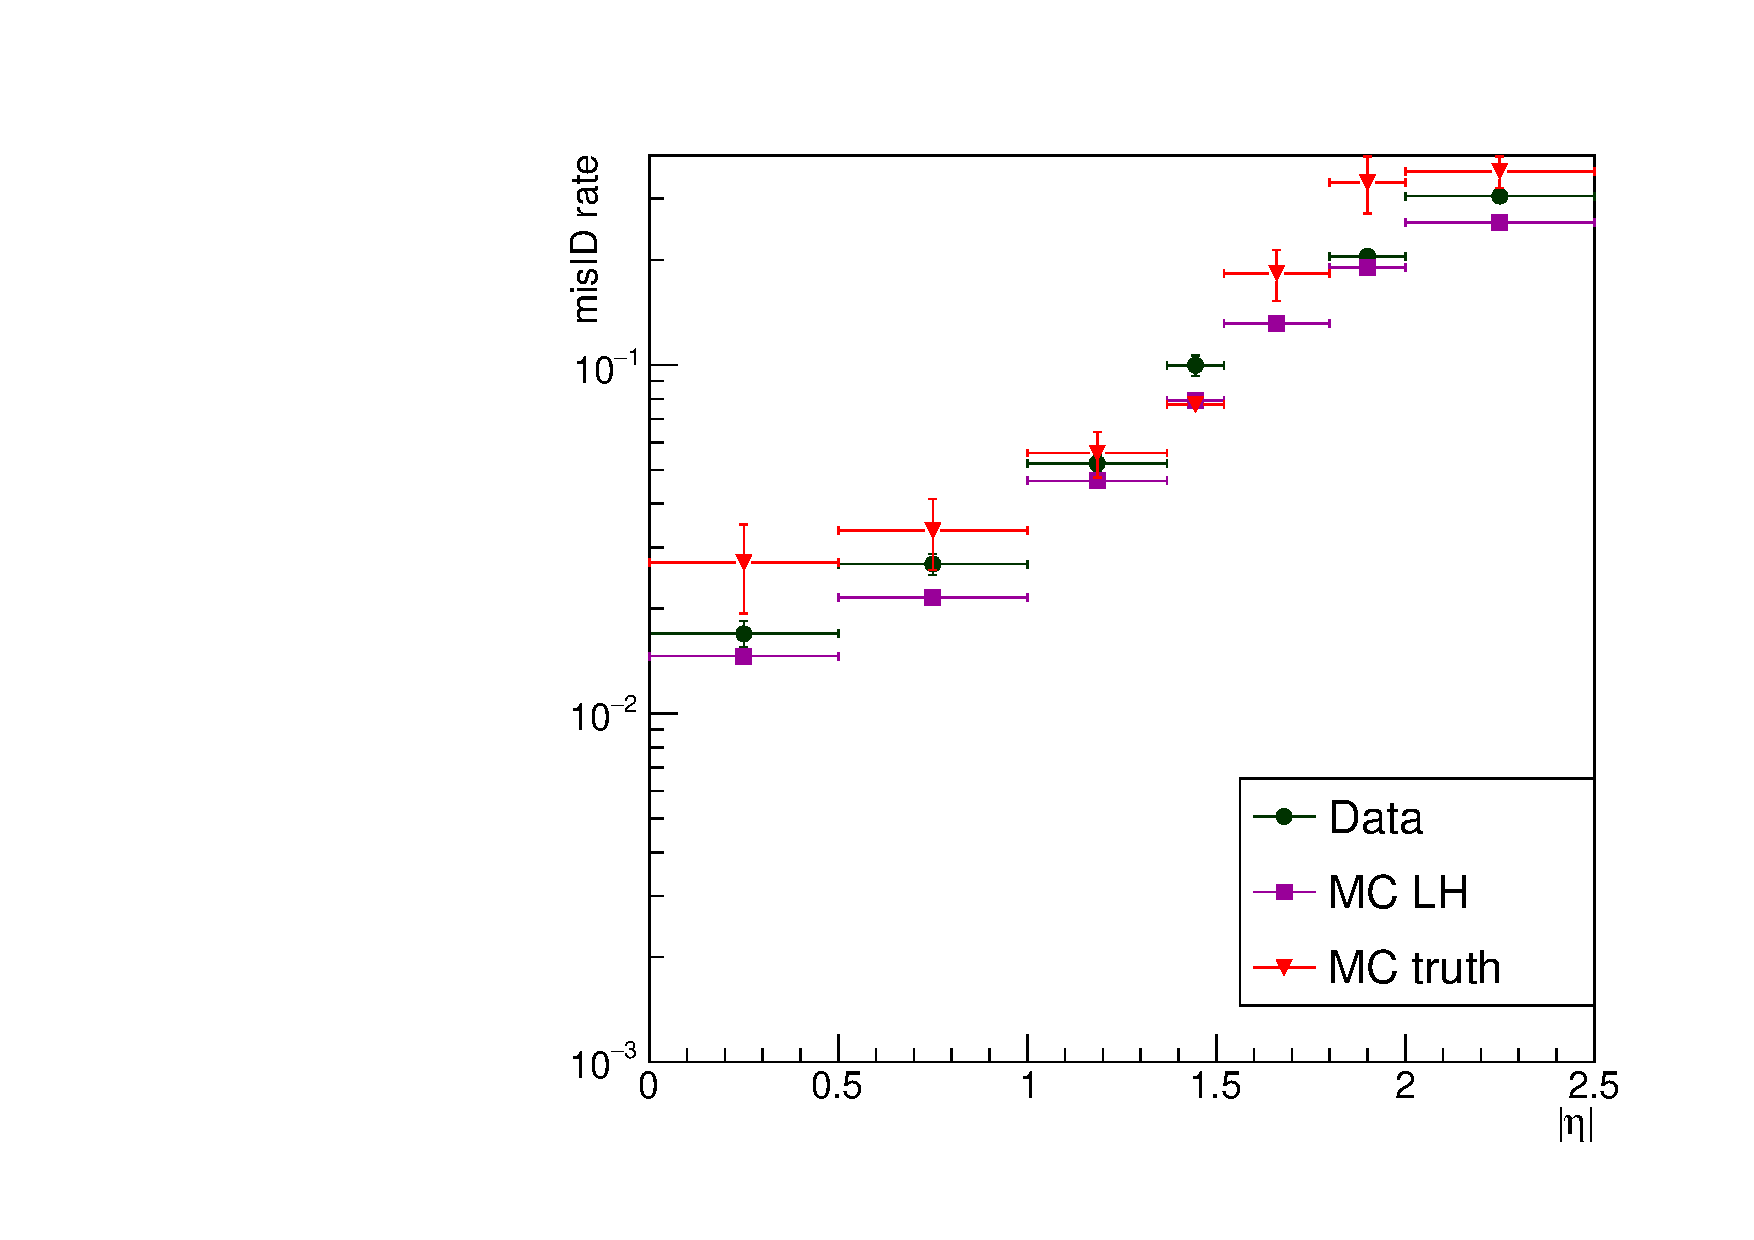
\includegraphics[scale=0.39]{ChargeMisID/WoSub_loose/Eta.pdf}}
\subfloat[][Comparison of rates for Signal electrons]{
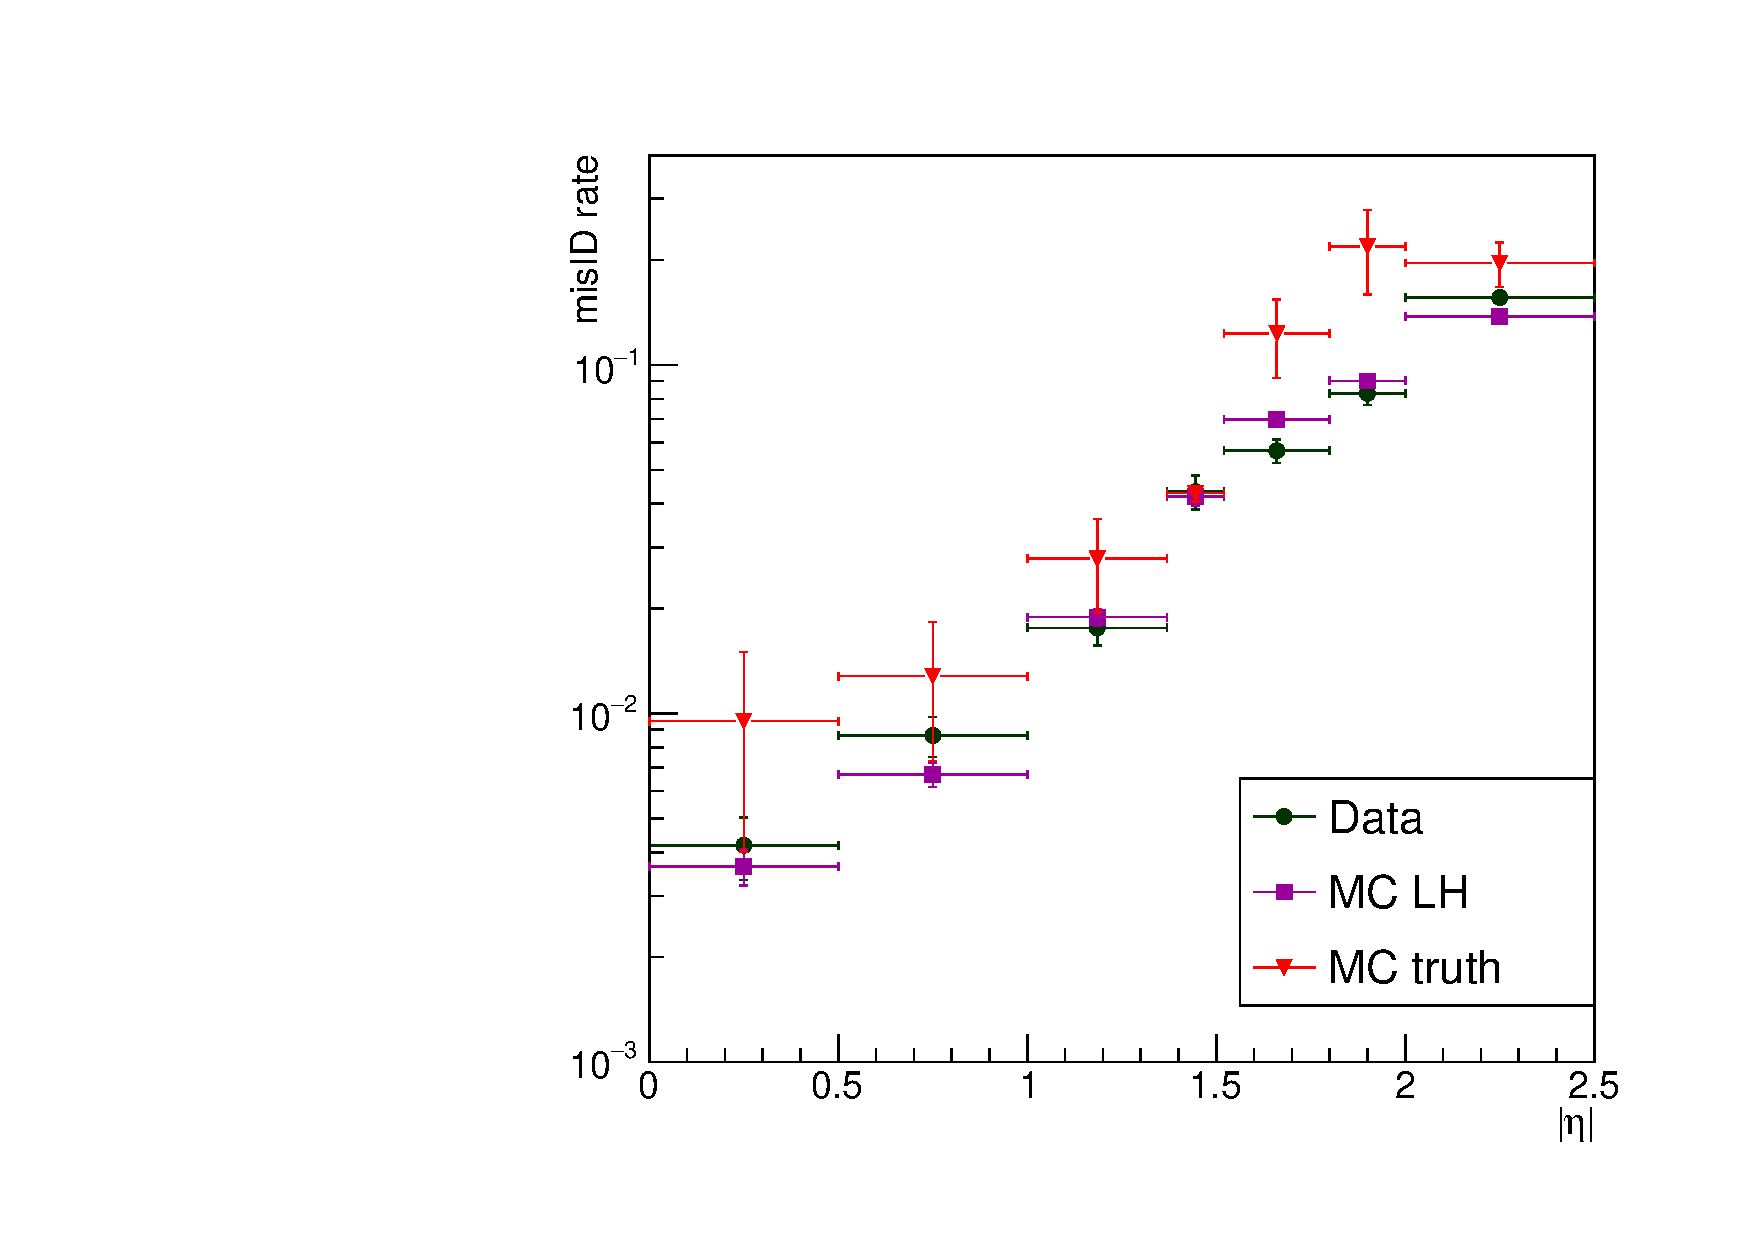
\includegraphics[scale=0.39]{ChargeMisID/WoSub_signal/Eta.pdf}}
\caption{Comparison of electron charge misidentification rates as a function of $|\eta|$}
\label{fig:rates-eta}
\end{figure}



Figures \ref{fig:rates-eta} and \ref{fig:rates-pt} compare the rates  obtained by the above methods for all $p_T$ ranges over $|\eta|$ and for all $|\eta|$ ranges over $p_T$ respectively. The full two-dimensional histograms showing the rates obtained by each method are figures \ref{fig:ChargeMisID-loose} and \ref{fig:ChargeMisID-signal} while plots showing the comparison of rates in each bin are figures \ref{fig:chargeMisID-CompareLoose} and \ref{fig:chargeMisID-CompareSignal}.

In general, the rates measured on data increase with $|\eta|$, which is as expected because the material budget of the detector increases with $|\eta|$ (Figure \ref{fig:material-budget}). 

The rates also rise gradually with $p_T$, which corresponds to electrons having straighter tracks, and thus a higher probability of being reconstructed with the wrong direction of curvature. There is an exception to this trend at $p_T\sim45$ GeV.

The rates obtained by the likelihood method on data and MC follow the same trends and generally agree with each other within reasonable limits. The differences can be attributed to the differences between the MC simulation and actual conditions inside the detector.

Figures \ref{fig:rates-eta} and \ref{fig:rates-pt} seem to suggest that the agreement between the MC truth and likelihood on MC do not agree well in all bins, especially at low $p_T$. However, further investigation into the comparisons in individual $|\eta|$ and $p_T$ bins show that they do, in fact, agree within reasonable limits. Thus the likelihood-based algorithm developed is shown to operate reasonably well and  provides reliable measurements when applied to data.

\newcommand{\TwoD}[2]{
  \makebox[\textwidth][c]{
  \begin{minipage}{1.15\textwidth}
  \subfloat[][#2]{\adjustbox{trim={0.02\width} {0.01\height} 0 {0.06\height},clip}%
    {\includegraphics[width=\textwidth]{#1}}
    }
  \end{minipage}} 
}

\begin{figure}[h]
\centering
\TwoD{ChargeMisID/WoSub_loose/hData.pdf}{Rates from likelihood on data}
\end{figure}

\begin{figure}[h]
\ContinuedFloat
\centering
\TwoD{ChargeMisID/WoSub_loose/hMCLH.pdf}{Rates from likelihood on MC}
\end{figure}

\begin{figure}[h]
\ContinuedFloat
\centering
\TwoD{ChargeMisID/WoSub_loose/hMC.pdf}{Rates from MC truth}
\caption{Charge misidentification rates for LooseBaseline electrons}
\label{fig:ChargeMisID-loose}
\end{figure}

\begin{figure}[h]
\centering
\TwoD{ChargeMisID/WoSub_signal/hData.pdf}{Rates from likelihood on data}
\end{figure}

\begin{figure}[h]
\ContinuedFloat
\centering
\TwoD{ChargeMisID/WoSub_signal/hMCLH.pdf}{Rates from likelihood on MC}
\end{figure}

\begin{figure}[h]
\ContinuedFloat
\centering
\TwoD{ChargeMisID/WoSub_signal/hMC.pdf}{Rates from MC truth}
\caption{Charge misidentification rates for Signal electrons}
\label{fig:ChargeMisID-signal}
\end{figure}

\begin{figure}[h]
\centering
\subfloat{
  \subfloat{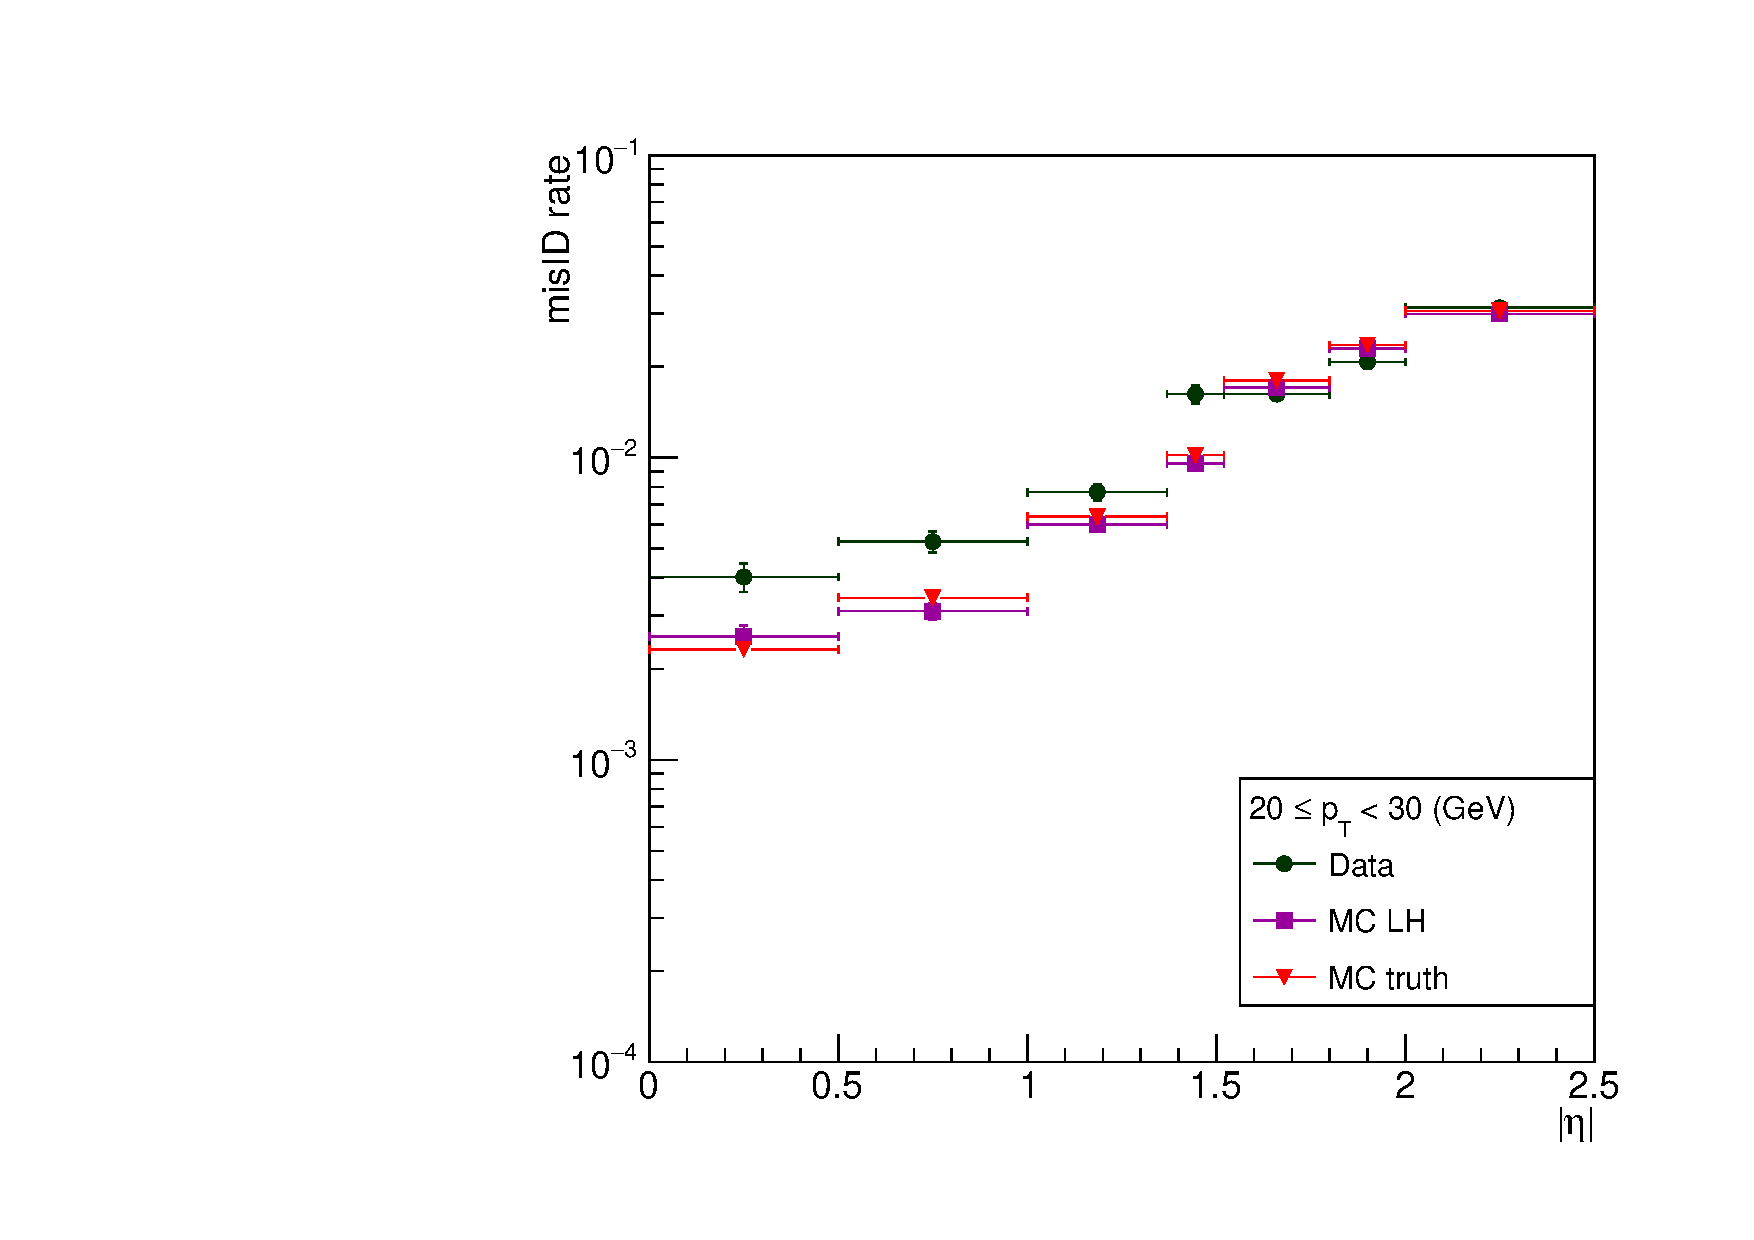
\includegraphics[page=1,scale=0.25]{ChargeMisID/WoSub_loose/EtaPt.pdf}}
  \subfloat{\includegraphics[page=2,scale=0.25]{ChargeMisID/WoSub_loose/EtaPt.pdf}}
  \subfloat{\includegraphics[page=3,scale=0.25]{ChargeMisID/WoSub_loose/EtaPt.pdf}}
}

\subfloat{
  \subfloat{\includegraphics[page=4,scale=0.25]{ChargeMisID/WoSub_loose/EtaPt.pdf}}
  \subfloat{\includegraphics[page=5,scale=0.25]{ChargeMisID/WoSub_loose/EtaPt.pdf}}
  \subfloat{\includegraphics[page=6,scale=0.25]{ChargeMisID/WoSub_loose/EtaPt.pdf}}
}

\subfloat{
  \subfloat{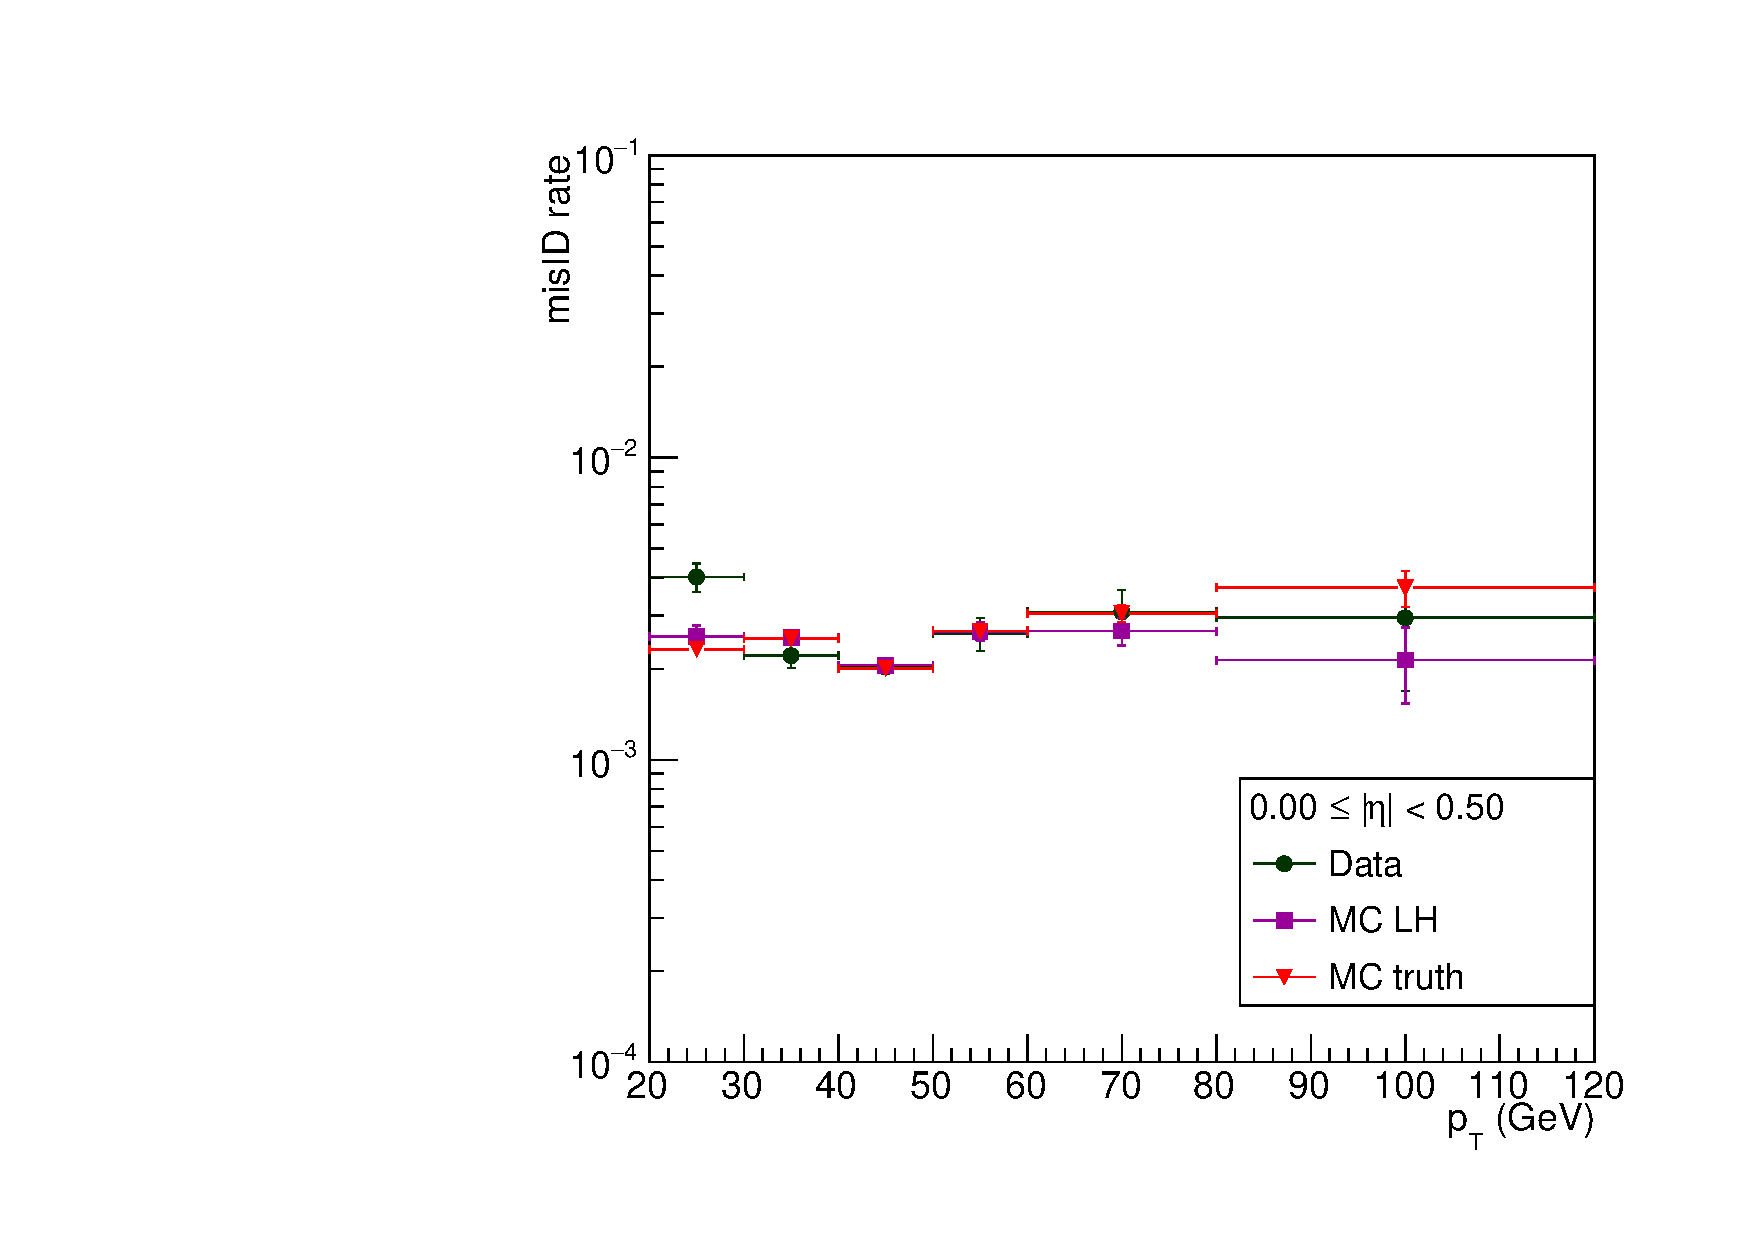
\includegraphics[page=1,scale=0.25]{ChargeMisID/WoSub_loose/PtEta.pdf}}
  \subfloat{\includegraphics[page=2,scale=0.25]{ChargeMisID/WoSub_loose/PtEta.pdf}}
  \subfloat{\includegraphics[page=3,scale=0.25]{ChargeMisID/WoSub_loose/PtEta.pdf}}
}

\subfloat{
  \subfloat{\includegraphics[page=5,scale=0.25]{ChargeMisID/WoSub_loose/PtEta.pdf}}
  \subfloat{\includegraphics[page=6,scale=0.25]{ChargeMisID/WoSub_loose/PtEta.pdf}}
  \subfloat{\includegraphics[page=7,scale=0.25]{ChargeMisID/WoSub_loose/PtEta.pdf}}
}
\caption[Comparison of charge misidentification rates for LooseBaseline electrons]{Comparison of charge misidentification rates for LooseBaseline electrons}
\label{fig:chargeMisID-CompareLoose}
\end{figure}

\begin{figure}[h]
\centering
\subfloat{
  \subfloat{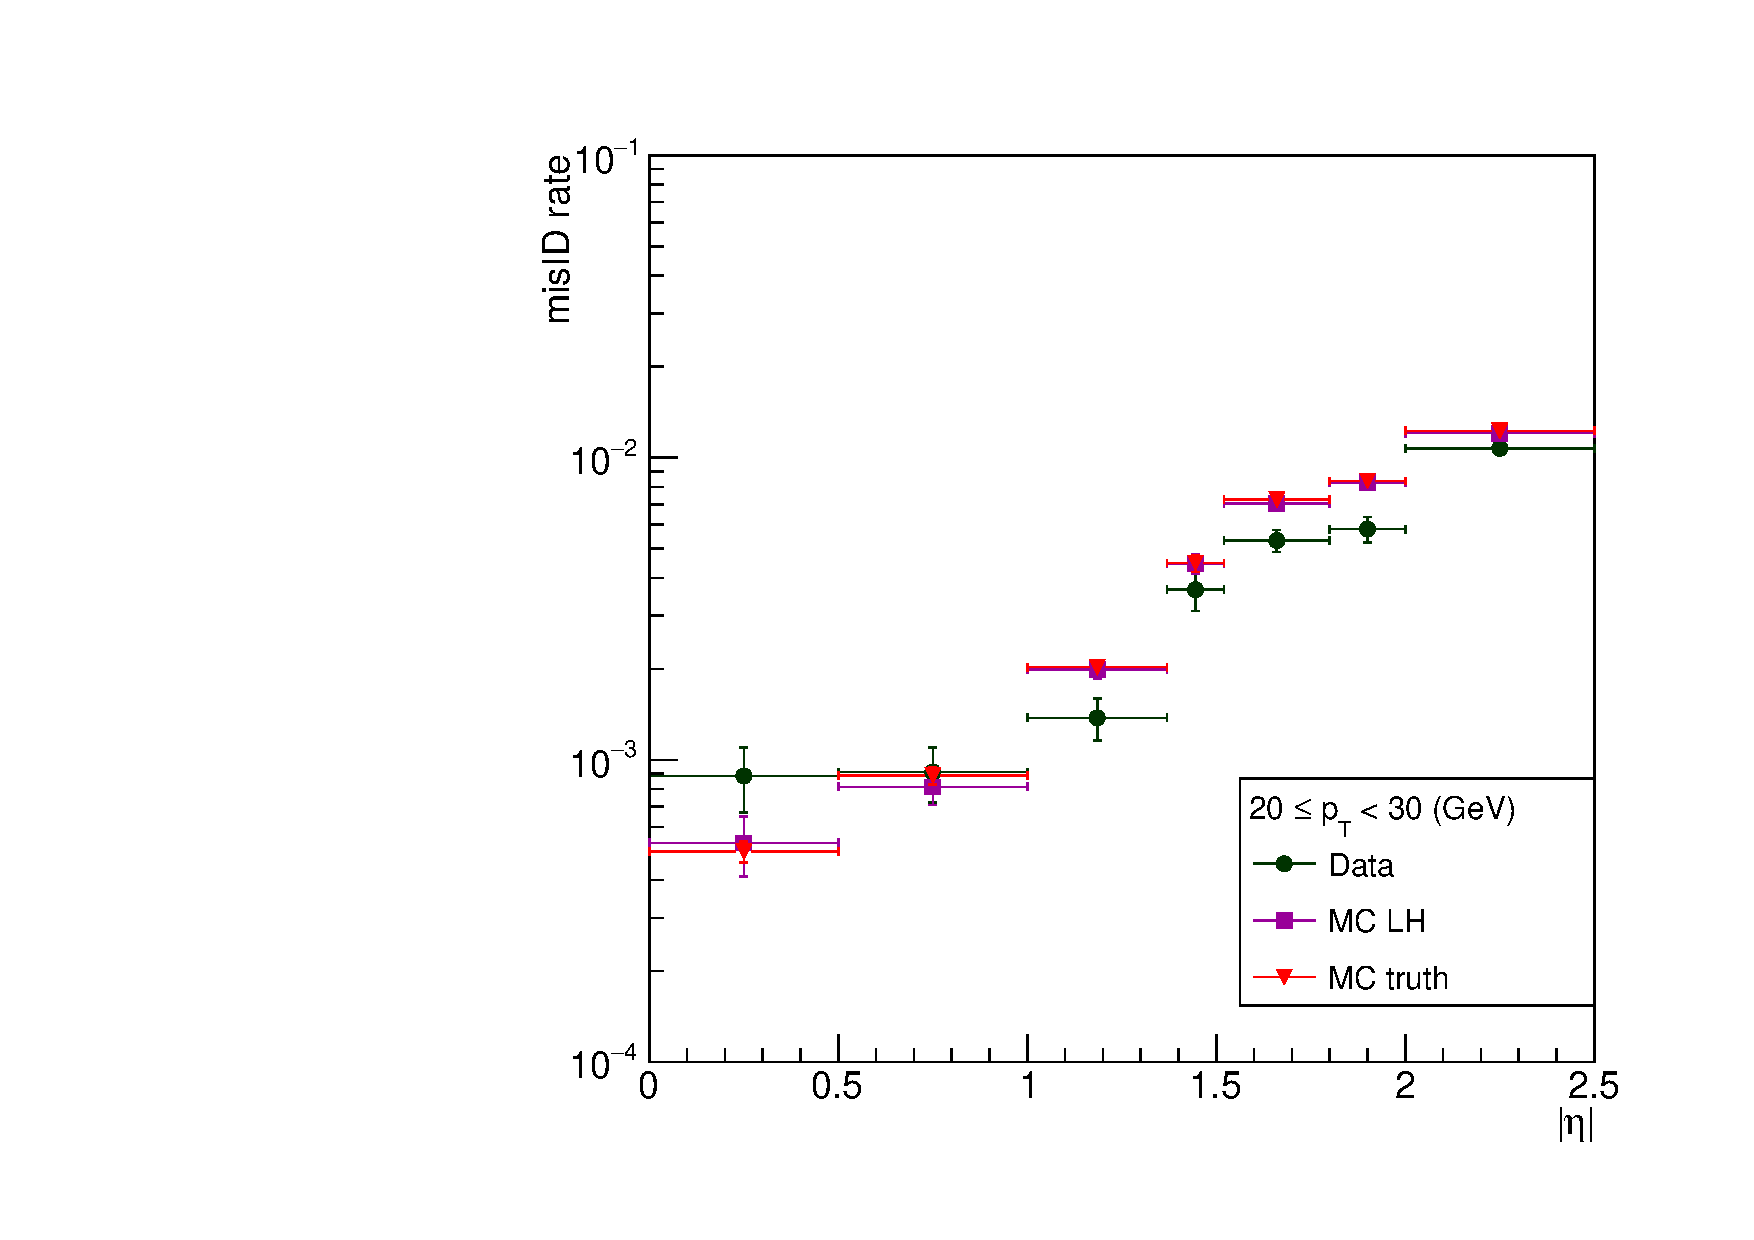
\includegraphics[page=1,scale=0.25]{ChargeMisID/WoSub_signal/EtaPt.pdf}}
  \subfloat{\includegraphics[page=2,scale=0.25]{ChargeMisID/WoSub_signal/EtaPt.pdf}}
  \subfloat{\includegraphics[page=3,scale=0.25]{ChargeMisID/WoSub_signal/EtaPt.pdf}}
}

\subfloat{
  \subfloat{\includegraphics[page=4,scale=0.25]{ChargeMisID/WoSub_signal/EtaPt.pdf}}
  \subfloat{\includegraphics[page=5,scale=0.25]{ChargeMisID/WoSub_signal/EtaPt.pdf}}
  \subfloat{\includegraphics[page=6,scale=0.25]{ChargeMisID/WoSub_signal/EtaPt.pdf}}
}

\subfloat{
  \subfloat{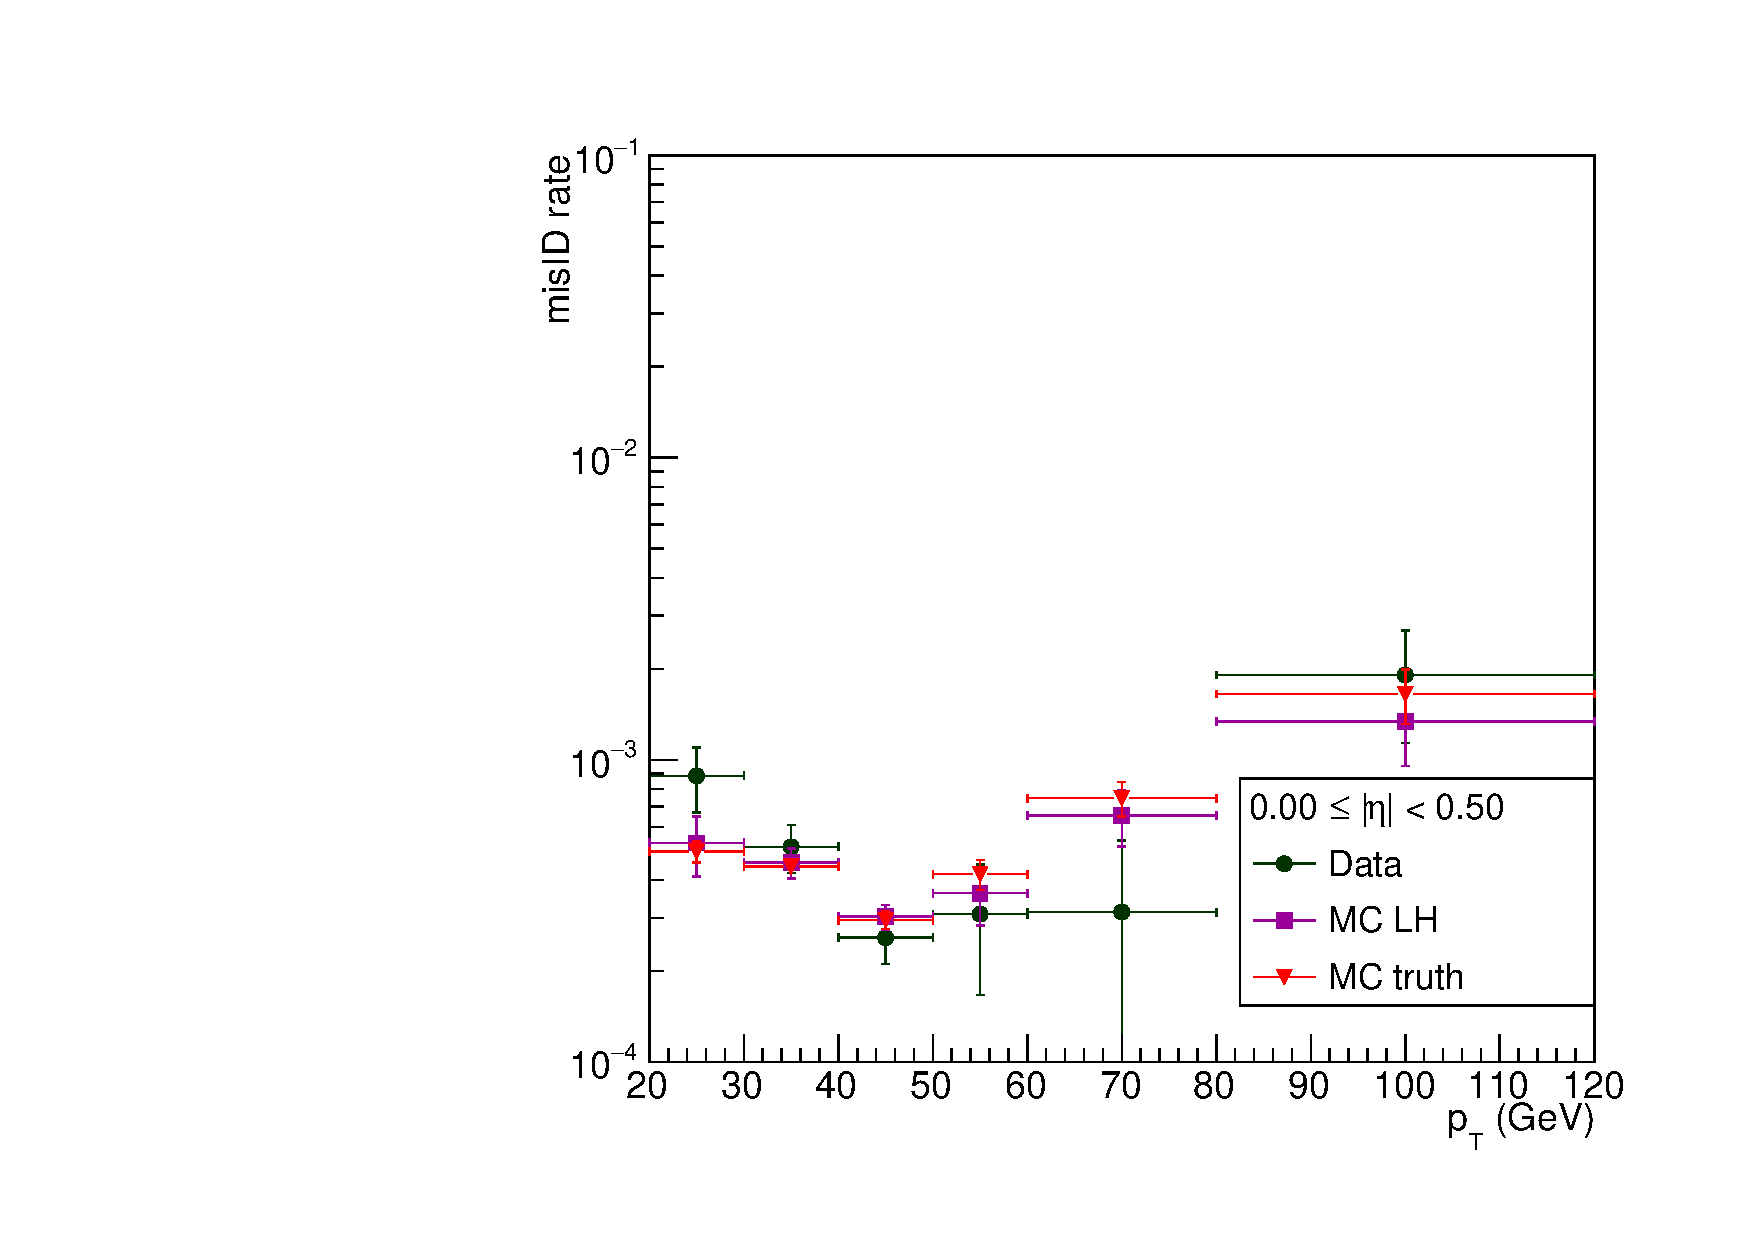
\includegraphics[page=1,scale=0.25]{ChargeMisID/WoSub_signal/PtEta.pdf}}
  \subfloat{\includegraphics[page=2,scale=0.25]{ChargeMisID/WoSub_signal/PtEta.pdf}}
  \subfloat{\includegraphics[page=3,scale=0.25]{ChargeMisID/WoSub_signal/PtEta.pdf}}
}

\subfloat{
  \subfloat{\includegraphics[page=5,scale=0.25]{ChargeMisID/WoSub_signal/PtEta.pdf}}
  \subfloat{\includegraphics[page=6,scale=0.25]{ChargeMisID/WoSub_signal/PtEta.pdf}}
  \subfloat{\includegraphics[page=7,scale=0.25]{ChargeMisID/WoSub_signal/PtEta.pdf}}
}
\caption[Comparison of charge misidentification rates for Signal electrons]{Comparison of charge misidentification rates for Signal electrons}
\label{fig:chargeMisID-CompareSignal}
\end{figure}

\FloatBarrier

\subsection{Summary}
The total background is summarised here, together with the systematic uncertainties.

%-------------------------------------------------------------------------------

\clearpage
%-------------------------------------------------------------------------------
\section{Control Region}
\label{sec:CR}
Data and MC samples are compared with different Z+jets MC samples with different generators.
The following Good Run List is used with total luminosity $3.3~\text{fb}^{-1}$:
\small
\begin{verbatim}
data15_13TeV.periodAllYear_DetStatus-v73-pro19-08_DQDefects-00-01-02_PHYS_StandardGRL_All_Good_25ns.xml
\end{verbatim}
\normalsize

The following data samples are used:
\small
\begin{verbatim}
data15_13TeV.00276262.physics_Main.merge.DAOD_SUSY2.f620_m1480_p2425/
data15_13TeV.00276329.physics_Main.merge.DAOD_SUSY2.f620_m1480_p2425/
data15_13TeV.00276336.physics_Main.merge.DAOD_SUSY2.f620_m1480_p2425/
data15_13TeV.00276416.physics_Main.merge.DAOD_SUSY2.f620_m1480_p2425/
data15_13TeV.00276511.physics_Main.merge.DAOD_SUSY2.f620_m1480_p2425/
data15_13TeV.00276689.physics_Main.merge.DAOD_SUSY2.f623_m1480_p2425/
data15_13TeV.00276778.physics_Main.merge.DAOD_SUSY2.f620_m1480_p2425/
data15_13TeV.00276790.physics_Main.merge.DAOD_SUSY2.f620_m1480_p2425/
data15_13TeV.00276952.physics_Main.merge.DAOD_SUSY2.f620_m1480_p2425/
data15_13TeV.00276954.physics_Main.merge.DAOD_SUSY2.f620_m1480_p2425/
data15_13TeV.00278880.physics_Main.merge.DAOD_SUSY2.f628_m1497_p2425/
data15_13TeV.00278912.physics_Main.merge.DAOD_SUSY2.f628_m1497_p2425/
data15_13TeV.00278968.physics_Main.merge.DAOD_SUSY2.f628_m1497_p2425/
data15_13TeV.00279169.physics_Main.merge.DAOD_SUSY2.f628_m1497_p2425/
data15_13TeV.00279259.physics_Main.merge.DAOD_SUSY2.f628_m1497_p2425/
data15_13TeV.00279279.physics_Main.merge.DAOD_SUSY2.f628_m1497_p2425/
data15_13TeV.00279284.physics_Main.merge.DAOD_SUSY2.f628_m1497_p2425/
data15_13TeV.00279345.physics_Main.merge.DAOD_SUSY2.f628_m1497_p2425/
data15_13TeV.00279515.physics_Main.merge.DAOD_SUSY2.f628_m1497_p2425/
data15_13TeV.00279598.physics_Main.merge.DAOD_SUSY2.f628_m1497_p2425/
data15_13TeV.00279685.physics_Main.merge.DAOD_SUSY2.f628_m1497_p2425/
data15_13TeV.00279764.physics_Main.merge.DAOD_SUSY2.f628_m1497_p2425/
data15_13TeV.00279813.physics_Main.merge.DAOD_SUSY2.f628_m1497_p2425/
data15_13TeV.00279867.physics_Main.merge.DAOD_SUSY2.f628_m1497_p2425/
data15_13TeV.00279928.physics_Main.merge.DAOD_SUSY2.f628_m1497_p2425/
data15_13TeV.00279932.physics_Main.merge.DAOD_SUSY2.f629_m1504_p2425/
data15_13TeV.00279984.physics_Main.merge.DAOD_SUSY2.f629_m1504_p2425/
data15_13TeV.00280231.physics_Main.merge.DAOD_SUSY2.f630_m1504_p2425/
data15_13TeV.00280319.physics_Main.merge.DAOD_SUSY2.f629_m1504_p2425/
data15_13TeV.00280368.physics_Main.merge.DAOD_SUSY2.f629_m1504_p2436/
data15_13TeV.00280423.physics_Main.merge.DAOD_SUSY2.f629_m1504_p2425/
data15_13TeV.00280464.physics_Main.merge.DAOD_SUSY2.f629_m1504_p2425/
data15_13TeV.00280500.physics_Main.merge.DAOD_SUSY2.f631_m1504_p2425/
data15_13TeV.00280520.physics_Main.merge.DAOD_SUSY2.f632_m1504_p2425/
data15_13TeV.00280614.physics_Main.merge.DAOD_SUSY2.f629_m1504_p2425/
data15_13TeV.00280673.physics_Main.merge.DAOD_SUSY2.f629_m1504_p2425/
data15_13TeV.00280753.physics_Main.merge.DAOD_SUSY2.f629_m1504_p2425/
data15_13TeV.00280853.physics_Main.merge.DAOD_SUSY2.f629_m1504_p2425/
data15_13TeV.00280862.physics_Main.merge.DAOD_SUSY2.f629_m1504_p2425/
data15_13TeV.00280950.physics_Main.merge.DAOD_SUSY2.f629_m1504_p2425/
data15_13TeV.00280977.physics_Main.merge.DAOD_SUSY2.f629_m1504_p2425/
data15_13TeV.00281070.physics_Main.merge.DAOD_SUSY2.f629_m1504_p2425/
data15_13TeV.00281074.physics_Main.merge.DAOD_SUSY2.f629_m1504_p2425/
data15_13TeV.00281075.physics_Main.merge.DAOD_SUSY2.f629_m1504_p2425/
data15_13TeV.00281317.physics_Main.merge.DAOD_SUSY2.f629_m1504_p2425/
data15_13TeV.00281385.physics_Main.merge.DAOD_SUSY2.f629_m1504_p2425/
data15_13TeV.00281411.physics_Main.merge.DAOD_SUSY2.f629_m1504_p2425/
data15_13TeV.00282625.physics_Main.merge.DAOD_SUSY2.f640_m1511_p2425/
data15_13TeV.00282631.physics_Main.merge.DAOD_SUSY2.f640_m1511_p2425/
data15_13TeV.00282712.physics_Main.merge.DAOD_SUSY2.f640_m1511_p2425/
data15_13TeV.00282784.physics_Main.merge.DAOD_SUSY2.f640_m1511_p2425/
data15_13TeV.00282992.physics_Main.merge.DAOD_SUSY2.f640_m1511_p2425/
data15_13TeV.00283074.physics_Main.merge.DAOD_SUSY2.f640_m1511_p2425/
data15_13TeV.00283155.physics_Main.merge.DAOD_SUSY2.f640_m1511_p2425/
data15_13TeV.00283270.physics_Main.merge.DAOD_SUSY2.f640_m1511_p2425/
data15_13TeV.00283429.physics_Main.merge.DAOD_SUSY2.f643_m1518_p2425/
data15_13TeV.00283608.physics_Main.merge.DAOD_SUSY2.f643_m1518_p2425/
data15_13TeV.00283780.physics_Main.merge.DAOD_SUSY2.f643_m1518_p2425/
data15_13TeV.00284006.physics_Main.merge.DAOD_SUSY2.f643_m1518_p2425/
data15_13TeV.00284154.physics_Main.merge.DAOD_SUSY2.f643_m1518_p2425/
data15_13TeV.00284213.physics_Main.merge.DAOD_SUSY2.f643_m1518_p2425/
data15_13TeV.00284285.physics_Main.merge.DAOD_SUSY2.f643_m1518_p2425/
data15_13TeV.00284420.physics_Main.merge.DAOD_SUSY2.f643_m1518_p2425/
data15_13TeV.00284427.physics_Main.merge.DAOD_SUSY2.f643_m1518_p2425/
data15_13TeV.00284484.physics_Main.merge.DAOD_SUSY2.f644_m1518_p2425/
\end{verbatim}
\normalsize

Z+jets samples generated by Powheg and MadGraph are compared, while other background MC samples are generated by Powheg.
The following MC samples are used for other background including $t\bar{t}$ and single top:
\scriptsize
\begin{verbatim}
mc15_13TeV.410000.PowhegPythiaEvtGen_P2012_ttbar_hdamp172p5_nonallhad.merge.DAOD_SUSY2.e3698_s2608_s2183_r6765_r6282_p2419/
mc15_13TeV.410015.PowhegPythiaEvtGen_P2012_Wt_dilepton_top.merge.DAOD_SUSY2.e3753_s2608_s2183_r6869_r6282_p2419/
mc15_13TeV.410016.PowhegPythiaEvtGen_P2012_Wt_dilepton_antitop.merge.DAOD_SUSY2.e3753_s2608_s2183_r6869_r6282_p2419/
\end{verbatim}
\normalsize

A signal MC sample is used for reference.
The following signal MC sample is used:
\scriptsize
\begin{verbatim}
mc15_13TeV.392200.MGPy8EG_A14N23LO_C1N2_WZ_350p0_250p0_3L_2L7.merge.DAOD_SUSY2.e4287_a766_a777_r6282_p2419/
\end{verbatim}
\normalsize

\subsection{pileup reweighting}
In this section, all background samples are reweighted according to pileup reweighting.
\subsubsection{Powheg samples}
The following Z+jets samples with Powheg generator are used:
\scriptsize
\begin{verbatim}
mc15_13TeV.361106.PowhegPythia8EvtGen_AZNLOCTEQ6L1_Zee.merge.DAOD_SUSY2.e3601_s2576_s2132_r6765_r6282_p2419/
mc15_13TeV.361107.PowhegPythia8EvtGen_AZNLOCTEQ6L1_Zmumu.merge.DAOD_SUSY2.e3601_s2576_s2132_r6765_r6282_p2419/
mc15_13TeV.361108.PowhegPythia8EvtGen_AZNLOCTEQ6L1_Ztautau.merge.DAOD_SUSY2.e3601_s2576_s2132_r6765_r6282_p2419/
\end{verbatim}
\normalsize

The comparisons for different variables are shown in Fig.~\ref{pileup_powheg_start}~-~\ref{pileup_powheg_end}.

There are great discrepancies between data and MC for mT2 variable.
The Powheg generator may not simulate the $\text{p}_{\text{T}}$ of Z very well, and the Z $\text{p}_{\text{T}}$ reweighting is done on the Z+jets samples in section~\ref{sec_zpt}.

\begin{figure}
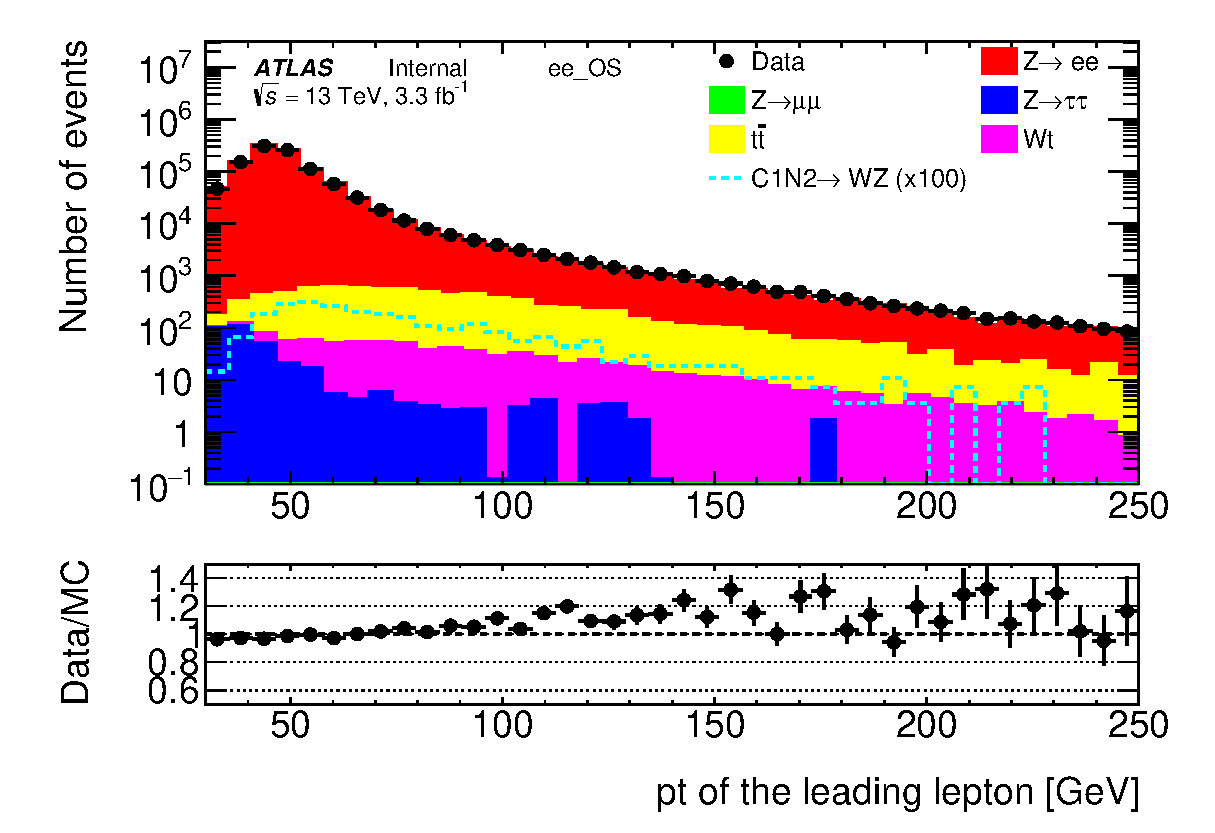
\includegraphics[width=0.5\textwidth]{CR/pileup_powheg/pt1_ee_OS}
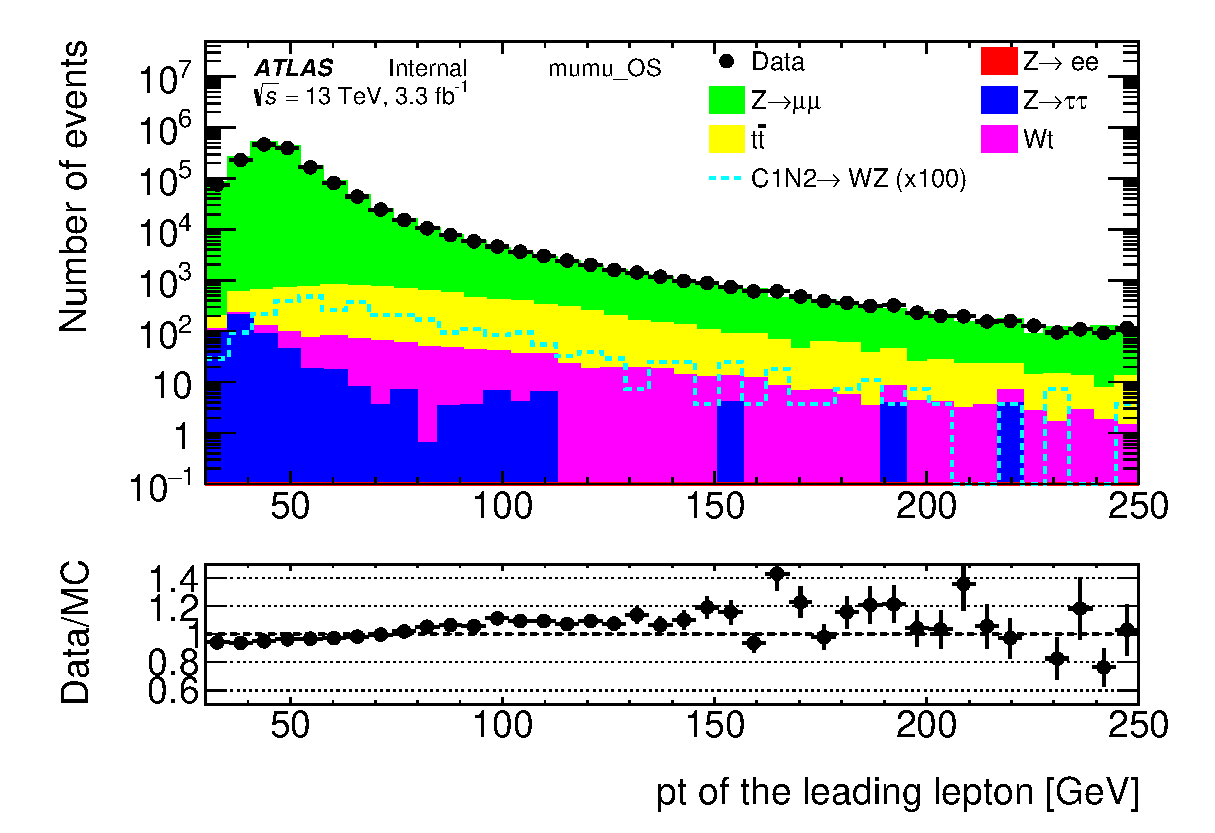
\includegraphics[width=0.5\textwidth]{CR/pileup_powheg/pt1_mumu_OS}
\caption{$\text{p}_{\text{T}}$ of the leading lepton for ee channel (left) and $\mu\mu$ channel (right).}
\label{pileup_powheg_start}
\end{figure}

\begin{figure}
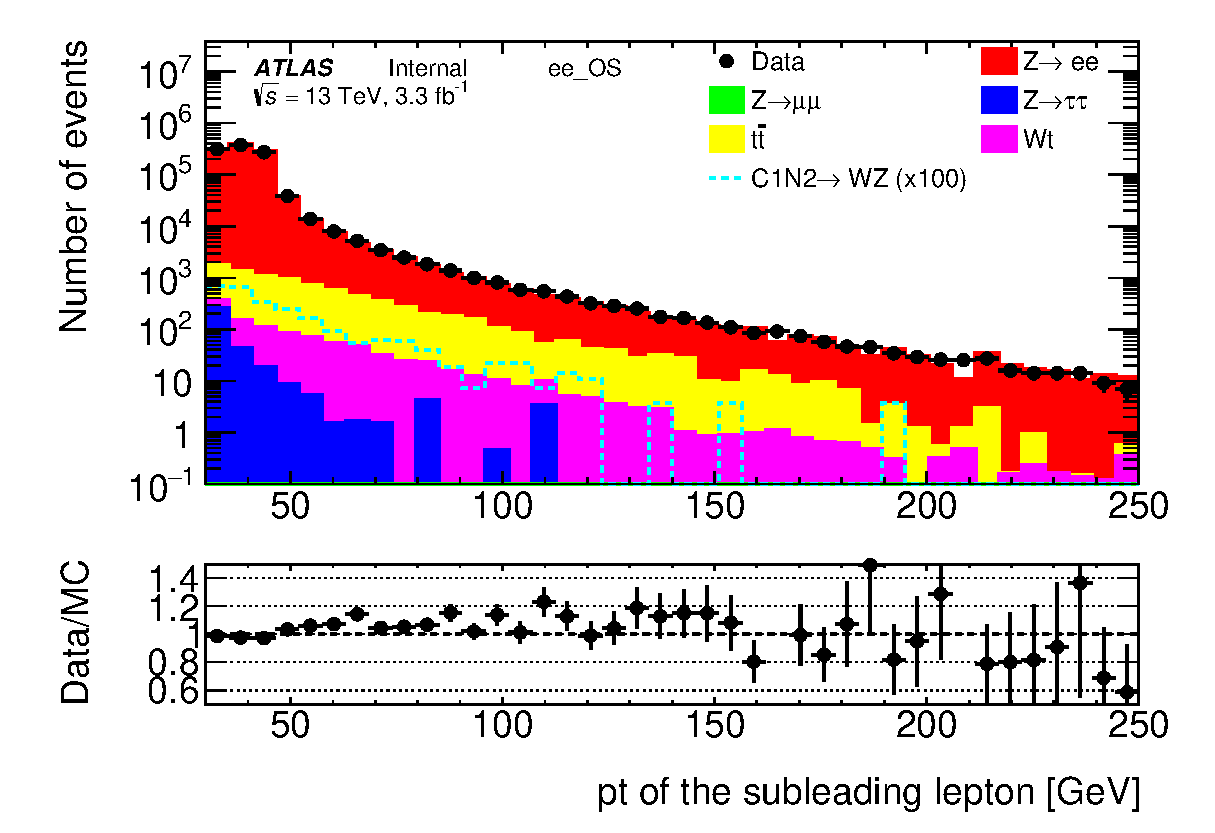
\includegraphics[width=0.5\textwidth]{CR/pileup_powheg/pt2_ee_OS}
\includegraphics[width=0.5\textwidth]{CR/pileup_powheg/pt2_mumu_OS}
\caption{$\text{p}_{\text{T}}$ of the subleading lepton for ee channel (left) and $\mu\mu$ channel (right).}
\end{figure}

\begin{figure}
\includegraphics[width=0.5\textwidth]{CR/pileup_powheg/mll_ee_OS}
\includegraphics[width=0.5\textwidth]{CR/pileup_powheg/mll_mumu_OS}
\caption{Dilepton invariant mass for ee channel (left) and $\mu\mu$ channel (right).}
\end{figure}

\begin{figure}
\includegraphics[width=0.5\textwidth]{CR/pileup_powheg/ptll_ee_OS}
\includegraphics[width=0.5\textwidth]{CR/pileup_powheg/ptll_mumu_OS}
\caption{Dilepton $\text{p}_{\text{T}}$ for ee channel (left) and $\mu\mu$ channel (right).}
\end{figure}

\begin{figure}
\includegraphics[width=0.5\textwidth]{CR/pileup_powheg/MET_ee_OS}
\includegraphics[width=0.5\textwidth]{CR/pileup_powheg/MET_mumu_OS}
\caption{MET for ee channel (left) and $\mu\mu$ channel (right).}
\end{figure}

\begin{figure}
\includegraphics[width=0.5\textwidth]{CR/pileup_powheg/mT2_ee_OS}
\includegraphics[width=0.5\textwidth]{CR/pileup_powheg/mT2_mumu_OS}
\caption{mT2 for ee channel (left) and $\mu\mu$ channel (right).}
\end{figure}

\begin{figure}
\includegraphics[width=0.5\textwidth]{CR/pileup_powheg/nJet_ee_OS}
\includegraphics[width=0.5\textwidth]{CR/pileup_powheg/nJet_mumu_OS}
\caption{Number of jets for ee channel (left) and $\mu\mu$ channel (right).}
\end{figure}

\begin{figure}
\includegraphics[width=0.5\textwidth]{CR/pileup_powheg/nBJet_ee_OS}
\includegraphics[width=0.5\textwidth]{CR/pileup_powheg/nBJet_mumu_OS}
\caption{Number of b-jets for ee channel (left) and $\mu\mu$ channel (right).}
\label{pileup_powheg_end}
\end{figure}

\subsubsection{MadGraph samples}
The following Z+jets samples with MadGraph generator are used:
\scriptsize
\begin{verbatim}
mc15_13TeV.361500.MadGraphPythia8EvtGen_A14NNPDF23LO_Zee_Np0.merge.DAOD_SUSY2.e3898_s2608_s2183_r6869_r6282_p2419/
mc15_13TeV.361501.MadGraphPythia8EvtGen_A14NNPDF23LO_Zee_Np1.merge.DAOD_SUSY2.e3898_s2608_s2183_r6869_r6282_p2419/
mc15_13TeV.361502.MadGraphPythia8EvtGen_A14NNPDF23LO_Zee_Np2.merge.DAOD_SUSY2.e3898_s2608_s2183_r6869_r6282_p2419/
mc15_13TeV.361503.MadGraphPythia8EvtGen_A14NNPDF23LO_Zee_Np3.merge.DAOD_SUSY2.e3898_s2608_s2183_r6869_r6282_p2419/
mc15_13TeV.361504.MadGraphPythia8EvtGen_A14NNPDF23LO_Zee_Np4.merge.DAOD_SUSY2.e3898_s2608_s2183_r6869_r6282_p2419/
mc15_13TeV.361505.MadGraphPythia8EvtGen_A14NNPDF23LO_Zmumu_Np0.merge.DAOD_SUSY2.e3898_s2608_s2183_r6869_r6282_p2419/
mc15_13TeV.361506.MadGraphPythia8EvtGen_A14NNPDF23LO_Zmumu_Np1.merge.DAOD_SUSY2.e3898_s2608_s2183_r6869_r6282_p2419/
mc15_13TeV.361507.MadGraphPythia8EvtGen_A14NNPDF23LO_Zmumu_Np2.merge.DAOD_SUSY2.e3898_s2608_s2183_r6869_r6282_p2419/
mc15_13TeV.361508.MadGraphPythia8EvtGen_A14NNPDF23LO_Zmumu_Np3.merge.DAOD_SUSY2.e3898_s2608_s2183_r6869_r6282_p2419/
mc15_13TeV.361509.MadGraphPythia8EvtGen_A14NNPDF23LO_Zmumu_Np4.merge.DAOD_SUSY2.e3898_s2608_s2183_r6869_r6282_p2419/
mc15_13TeV.361510.MadGraphPythia8EvtGen_A14NNPDF23LO_Ztautau_Np0.merge.DAOD_SUSY2.e3898_s2608_s2183_r6869_r6282_p2419/
mc15_13TeV.361511.MadGraphPythia8EvtGen_A14NNPDF23LO_Ztautau_Np1.merge.DAOD_SUSY2.e3898_s2608_s2183_r6869_r6282_p2419/
mc15_13TeV.361512.MadGraphPythia8EvtGen_A14NNPDF23LO_Ztautau_Np2.merge.DAOD_SUSY2.e3898_s2608_s2183_r6869_r6282_p2419/
mc15_13TeV.361513.MadGraphPythia8EvtGen_A14NNPDF23LO_Ztautau_Np3.merge.DAOD_SUSY2.e3898_s2608_s2183_r6869_r6282_p2419/
mc15_13TeV.361514.MadGraphPythia8EvtGen_A14NNPDF23LO_Ztautau_Np4.merge.DAOD_SUSY2.e3898_s2608_s2183_r6869_r6282_p2419/
\end{verbatim}
\normalsize

The comparisons for different variables are shown in Fig.~\ref{pileup_MadGraph_start}~-~\ref{pileup_MadGraph_end}.

\begin{figure}
\includegraphics[width=0.5\textwidth]{CR/pileup_MadGraph/pt1_ee_OS}
\includegraphics[width=0.5\textwidth]{CR/pileup_MadGraph/pt1_mumu_OS}
\caption{$\text{p}_{\text{T}}$ of the leading lepton for ee channel (left) and $\mu\mu$ channel (right).}
\label{pileup_MadGraph_start}
\end{figure}

\begin{figure}
\includegraphics[width=0.5\textwidth]{CR/pileup_MadGraph/pt2_ee_OS}
\includegraphics[width=0.5\textwidth]{CR/pileup_MadGraph/pt2_mumu_OS}
\caption{$\text{p}_{\text{T}}$ of the subleading lepton for ee channel (left) and $\mu\mu$ channel (right).}
\end{figure}

\begin{figure}
\includegraphics[width=0.5\textwidth]{CR/pileup_MadGraph/mll_ee_OS}
\includegraphics[width=0.5\textwidth]{CR/pileup_MadGraph/mll_mumu_OS}
\caption{Dilepton invariant mass for ee channel (left) and $\mu\mu$ channel (right).}
\end{figure}

\begin{figure}
\includegraphics[width=0.5\textwidth]{CR/pileup_MadGraph/ptll_ee_OS}
\includegraphics[width=0.5\textwidth]{CR/pileup_MadGraph/ptll_mumu_OS}
\caption{Dilepton $\text{p}_{\text{T}}$ for ee channel (left) and $\mu\mu$ channel (right).}
\end{figure}

\begin{figure}
\includegraphics[width=0.5\textwidth]{CR/pileup_MadGraph/MET_ee_OS}
\includegraphics[width=0.5\textwidth]{CR/pileup_MadGraph/MET_mumu_OS}
\caption{MET for ee channel (left) and $\mu\mu$ channel (right).}
\end{figure}

\begin{figure}
\includegraphics[width=0.5\textwidth]{CR/pileup_MadGraph/mT2_ee_OS}
\includegraphics[width=0.5\textwidth]{CR/pileup_MadGraph/mT2_mumu_OS}
\caption{mT2 for ee channel (left) and $\mu\mu$ channel (right).}
\end{figure}

\begin{figure}
\includegraphics[width=0.5\textwidth]{CR/pileup_MadGraph/nJet_ee_OS}
\includegraphics[width=0.5\textwidth]{CR/pileup_MadGraph/nJet_mumu_OS}
\caption{Number of jets for ee channel (left) and $\mu\mu$ channel (right).}
\end{figure}

\begin{figure}
\includegraphics[width=0.5\textwidth]{CR/pileup_MadGraph/nBJet_ee_OS}
\includegraphics[width=0.5\textwidth]{CR/pileup_MadGraph/nBJet_mumu_OS}
\caption{Number of b-jets for ee channel (left) and $\mu\mu$ channel (right).}
\label{pileup_MadGraph_end}
\end{figure}

\clearpage
\subsection{Z $\text{p}_{\text{T}}$ reweighting}
\label{sec_zpt}
In this section, the Z $\text{p}_{\text{T}}$ reweighting, in addition to the pileup reweighting, is done on the Z+jets samples generated by Powheg.
The ratio of the number of Z+jets events from data to that from Z+jets MC is calculated by
\begin{equation}
\text{Ratio} = \frac{\text{(Data)}-\text{(MC of non Z+jets)}}{\text{(MC of Z+jets)}}
\end{equation}
Two different methods of fitting are used: simple fit and combined fit.

\subsubsection{Simple fit}
For the simple fit, the ratio plots are fitted by second order polynomials $y = a_0 + a_1 x + a_2 x^2$ independently.
The plots of the ratio against dilepton $\text{p}_{\text{T}}$ for ee and $\mu\mu$ channel are shown in Fig.~\ref{zpt_powheg_simple}.
\begin{figure}
\centering
\includegraphics[width=0.5\textwidth]{CR/Zpt_powheg_simple/ptll_rw}
\caption{The plots of ratio against dilepton $\text{p}_{\text{T}}$ for ee channel (black) and $\mu\mu$ channel (red).}
\label{zpt_powheg_simple}
\end{figure}
For ee channel, the fitting results are
\begin{equation}
a_0 = 0.968 \pm 0.003 \qquad
a_1 = (3.2 \pm 1.8) \times 10^{-4} \qquad
a_2 = (7.1 \pm 1.6) \times 10^{-6}
\end{equation}
For $\mu\mu$ channel, the fitting results are
\begin{equation}
a_0 = 0.940 \pm 0.002 \qquad
a_1 = (7.9 \pm 1.5) \times 10^{-4} \qquad
a_2 = (3.3 \pm 1.3) \times 10^{-6}
\end{equation}
The dilepton $\text{p}_{\text{T}}$ and mT2 are then reweighted according to the corresponding channel and their dilepton $\text{p}_{\text{T}}$.
The reweighted plots for dilepton $\text{p}_{\text{T}}$ and mT2 are shown in Fig.~\ref{zpt_powheg_simple_start}~-~\ref{zpt_powheg_simple_end}.

\begin{figure}
\includegraphics[width=0.5\textwidth]{CR/Zpt_powheg_simple/ptll_ee_OS}
\includegraphics[width=0.5\textwidth]{CR/Zpt_powheg_simple/ptll_mumu_OS}
\caption{Dilepton $\text{p}_{\text{T}}$ for ee channel (left) and $\mu\mu$ channel (right).}
\label{zpt_powheg_simple_start}
\end{figure}

\begin{figure}
\includegraphics[width=0.5\textwidth]{CR/Zpt_powheg_simple/mT2_ee_OS}
\includegraphics[width=0.5\textwidth]{CR/Zpt_powheg_simple/mT2_mumu_OS}
\caption{mT2 for ee channel (left) and $\mu\mu$ channel (right).}
\label{zpt_powheg_simple_end}
\end{figure}

\subsubsection{Combined fit}
For the combined fit, the ratio plot for the $\mu\mu$ channel is fitted by a second order polynomial $y = a_0 + a_1 x + a_2 x^2$, while the ratio plot for the ee channel is fitted by another second order polynomial with one more scale factor $c$, $y = c(a_0 + a_1 x + a_2 x^2)$.
The plots of the ratio against dilepton $\text{p}_{\text{T}}$ for ee and $\mu\mu$ channel are shown in Fig.~\ref{zpt_powheg_combined}.
\begin{figure}
\centering
\includegraphics[width=0.5\textwidth]{CR/Zpt_powheg_combined/ptll_rw}
\caption{The plots of ratio against dilepton $\text{p}_{\text{T}}$ for ee channel (black) and $\mu\mu$ channel (red).}
\label{zpt_powheg_combined}
\end{figure}
The fitting results are
\begin{equation}
a_0 = 0.942 \pm 0.002 \qquad
a_1 = (5.9 \pm 1.1) \times 10^{-4} \qquad
a_2 = (4.8 \pm 1.0) \times 10^{-6} \qquad
c =  1.023 \pm 0.002
\end{equation}
The dilepton $\text{p}_{\text{T}}$ and mT2 are then reweighted according to the fitting function of the $\mu\mu$ channel and their dilepton $\text{p}_{\text{T}}$.
The reweighted plots for dilepton $\text{p}_{\text{T}}$ and mT2 are shown in Fig.~\ref{zpt_powheg_combined_start}~-~\ref{zpt_powheg_combined_end}.

\begin{figure}
\includegraphics[width=0.5\textwidth]{CR/Zpt_powheg_combined/ptll_ee_OS}
\includegraphics[width=0.5\textwidth]{CR/Zpt_powheg_combined/ptll_mumu_OS}
\caption{Dilepton $\text{p}_{\text{T}}$ for ee channel (left) and $\mu\mu$ channel (right).}
\label{zpt_powheg_combined_start}
\end{figure}

\begin{figure}
\includegraphics[width=0.5\textwidth]{CR/Zpt_powheg_combined/mT2_ee_OS}
\includegraphics[width=0.5\textwidth]{CR/Zpt_powheg_combined/mT2_mumu_OS}
\caption{mT2 for ee channel (left) and $\mu\mu$ channel (right).}
\label{zpt_powheg_combined_end}
\end{figure}

%-------------------------------------------------------------------------------

\clearpage
%-------------------------------------------------------------------------------
\section{Results}
\label{sec:results}
%\input{chapters/susy2lSS-results}
\subsection{Standard Model Test}
Compare data and background.

\subsection{Limits of New Physics}
Limits set for new physics.

%-------------------------------------------------------------------------------

%-------------------------------------------------------------------------------
\section{Conclusion}
\label{sec:conclusion}
%  \input{chapters/susy2lSS-conclusion}
%-------------------------------------------------------------------------------
Place your conclusion here.


%-------------------------------------------------------------------------------
\section*{Acknowledgements}
%-------------------------------------------------------------------------------

%\input{acknowledgements/Acknowledgements}

The \texttt{atlaslatex} package contains the acknowledgements that were valid 
at the time of the release you are using. These can be found in the
\texttt{acknowledgements} subdirectory.
When your ATLAS papers or CONF note is ready to be published,
download the latest set of acknowledgements from:\\
\url{https://twiki.cern.ch/twiki/bin/view/AtlasProtected/PubComAcknowledgements}

The supporting notes for the analysis should also contain a list of contributors.
This information should usually be included in \texttt{mydocument-metadata.tex}.
The list should be printed either here or before the table of contents.


%-------------------------------------------------------------------------------
\clearpage
\appendix
\part*{Appendix}
\addcontentsline{toc}{part}{Appendix}
\section{Comparison of isolation efficiency for AF2 and full simulation}
\label{app_AF2_iso}

The signal samples are produced using fast simulation, while the performance studies are mainly using fully simulated samples.

Following samples are used to compare the two simulation:
\scriptsize
\begin{verbatim}
mc15_13TeV.392216.MGPy8EG_A14N23LO_C1N2_WZ_450p0_50p0_3L_2L7.merge.DAOD_SUSY2.e4287_s2608_s2183_r6869_r6282_p2419
mc15_13TeV.392216.MGPy8EG_A14N23LO_C1N2_WZ_450p0_50p0_3L_2L7.merge.DAOD_SUSY2.e4287_a766_a777_r6282_p2419
\end{verbatim}
\normalsize

Good agreement of AF2 and full simulation is observed as shown below.
\subsection{Electron isolation}
The isolation variables are shown in Fig.~\ref{fig_el_isovar}. The efficiency comparison for eight electron isolation working points is shown in Fig.~\ref{fig_el_isoeff}.

\begin{figure}
\includegraphics[width=0.5\textwidth]{app/electron_topoetcone20_log}
\includegraphics[width=0.5\textwidth]{app/electron_ptvarcone30} 
\caption{Electron isolation variables.}
\label{fig_el_isovar}
\end{figure}

\begin{figure}
\includegraphics[width=0.5\textwidth]{app/electron_Loose}
\includegraphics[width=0.5\textwidth]{app/electron_Tight}
\includegraphics[width=0.5\textwidth]{app/electron_Gradient}
\includegraphics[width=0.5\textwidth]{app/electron_GradientLoose}
\includegraphics[width=0.5\textwidth]{app/electron_FixedCutLoose}
\includegraphics[width=0.5\textwidth]{app/electron_FixedCutTight}
\includegraphics[width=0.5\textwidth]{app/electron_LooseTrackOnly}
\includegraphics[width=0.5\textwidth]{app/electron_FixedCutTightTrackOnly}
\caption{Electron isolation efficiency comparison.}
\label{fig_el_isoeff}
\end{figure}


\subsection{Muon isolation}
The muon isolation variables are shown in Fig.~\ref{fig_muon_isovar}.
The efficiency comparison for seven muon isolation working points is shown in Fig.~\ref{fig_muon_isoeff}.

\begin{figure}
\includegraphics[width=0.5\textwidth]{app/muon_topoetcone20}
\includegraphics[width=0.5\textwidth]{app/muon_ptvarcone30}
\caption{Muon isolation variables.}
\label{fig_muon_isovar}
\end{figure}

\begin{figure}
\includegraphics[width=0.5\textwidth]{app/muon_Loose}
\includegraphics[width=0.5\textwidth]{app/muon_Tight}
\includegraphics[width=0.5\textwidth]{app/muon_Gradient}
\includegraphics[width=0.5\textwidth]{app/muon_GradientLoose}
\includegraphics[width=0.5\textwidth]{app/muon_FixedCutLoose}
\includegraphics[width=0.5\textwidth]{app/muon_LooseTrackOnly}
\includegraphics[width=0.5\textwidth]{app/muon_FixedCutTightTrackOnly}
\caption{Muon isolation efficiency comparison.}
\label{fig_muon_isoeff}
\end{figure}



\clearpage
\section{Cut based sensitivity study}
These studies are done using the \verb+p2879+ SUSY2 derivation samples for background and \verb+2949+ for signal.

\subsection{Taggetted signal}
The compressed region with 50~\GeV\ or 100~\GeV\ mass splitting.

\subsection{Background}
The considered background including
\begin{itemize}
  \item Di-boson\\
    Same sign $WW$, $WZ$ and $ZZ$ with one or two leptons undetected are inreducible background. $t\bar{t}V$ with one lepton from top quark and the other one from boson. $W+\gamma$ with the photon mis-identified as electron and the other one from $W$ decay.
  \item Charge flip of OS events\\
    Mainly for electrons. The electron has bremsstrahlung inside the detector and the emitted photon coverted to electron-positron pair. The opposite sign lepton is reconstructed thus give a same-sign pair with another lepton.
  \item Jet mis-identified as electron or muon.\\
    The rate for jet to be mis-reconstructed as electron is larger than muon.
\end{itemize}

\subsection{Method}

\subsection{Results}

\subsection{Conclusion}
Conclusion

\section{Multivariable analysis}

\subsection{Samples}
Signal samples:
\begin{itemize}
\item mc15\_13TeV.392415.MGPy8EG\_A14N23LO\_C1N2\_Slep\_400\_300\_0p95\_2L5.merge.DAOD\_SUSY2.e4287\_a766\_a810\_r6282\_p2499\_p2500\_pUM999999
\end{itemize}

Background samples:

Charge flip and fake lepton background are data driven. The GRL $data16_13TeV.periodAllYear\_DetStatus-v823-pro20-15\_DQDefects-00-02-04\_PHYS\_StandardGRL\_All\_Good_25ns.xml$ was used. The 33.26fb-1 data used covers run 297730 to 311481

%FIXME,  should not have a separate section for BDT evt selection, bkg and trig
Wgamma, diboson and ttbar background are from following MC samples:\\
\begin{itemize}
\item 410066	MadGraphPythia8EvtGen\_A14NNPDF23LO\_ttW\_Np0
\item 410067	MadGraphPythia8EvtGen\_A14NNPDF23LO\_ttW\_Np1
\item 410068	MadGraphPythia8EvtGen\_A14NNPDF23LO\_ttW\_Np2
\item 410112	MadGraphPythia8EvtGen\_A14NNPDF23LO\_ttee\_Np1
\item 410115	MadGraphPythia8EvtGen\_A14NNPDF23LO\_tttautau\_Np0
\item 410114	MadGraphPythia8EvtGen\_A14NNPDF23LO\_ttmumu\_Np1
\item 410113	MadGraphPythia8EvtGen\_A14NNPDF23LO\_ttmumu\_Np0
\item 410111	MadGraphPythia8EvtGen\_A14NNPDF23LO\_ttee\_Np0
\item 410116	MadGraphPythia8EvtGen\_A14NNPDF23LO\_tttautau\_Np1
\item 361063	Sherpa\_CT10\_llll
\item 361064	Sherpa\_CT10\_lllvSFMinus
\item 361065	Sherpa\_CT10\_lllvOFMinus
\item 361066	Sherpa\_CT10\_lllvSFPlus
\item 361067	Sherpa\_CT10\_lllvOFPlus
\item 361068	Sherpa\_CT10\_llvv
\item 361069	Sherpa\_CT10\_llvvjj\_ss\_EW4
\item 361070	Sherpa\_CT10\_llvvjj\_ss\_EW6
\item 361071	Sherpa\_CT10\_lllvjj\_EW6
\item 361072	Sherpa\_CT10\_lllljj\_EW6
\item 301890	Sherpa\_CT10\_enugammaPt35\_70
\item 301891	Sherpa\_CT10\_enugammaPt70\_140
\item 301892	Sherpa\_CT10\_enugammaPt140
\item 301893	Sherpa\_CT10\_munugammaPt35\_70
\item 301894	Sherpa\_CT10\_munugammaPt70\_140
\item 301895	Sherpa\_CT10\_munugammaPt140
\item 301896	Sherpa\_CT10\_taunugammaPt35\_70
\item 301897	Sherpa\_CT10\_taunugammaPt70\_140
\item 301898	Sherpa\_CT10\_taunugammaPt140
\end{itemize}

Data Selection:\\
The follow filters are applied to the data 
\begin{description}


\item [nPrimaryVertex>0] a Vertex need 2+ tracks with pT 2+GeV to be accepted as a primaryVertex
\item [GRL]
\item [“Standard” object definition] \ \\
Tight e TightLLH, Et<20GeV, eta<2.47 \\
Tight mu Medium, pT<25GeV, eta<2.7 \\
and others\\

\item [Exactly 2 lepton]
\item [triggerCut] \ \\

muonTrig =["HLT\_mu26\_imedium", "HLT\_mu24\_imedium", "HLT\_mu24\_iloose\_L1MU15","HLT\_mu20\_iloose\_L1MU15", "HLT\_mu50", "HLT\_mu60\_0eta105\_msonly"]\\

dimuonTrig = ["HLT\_2mu14","HLT\_2mu10","HLT\_mu24\_mu8noL1","HLT\_mu22\_mu8noL1","HLT\_mu20\_mu8noL1","HLT\_mu18\_mu8noL1"]\\

trimuonTrig = ["HLT\_mu24\_2mu4noL1","HLT\_mu22\_2mu4noL1","HLT\_mu20\_2mu4noL1","HLT\_mu18\_2mu4noL1","HLT\_3mu6","HLT\_3mu6\_msonly"]\\

electronTrigCut = ["HLT\_e26\_tight\_iloose","HLT\_e60\_medium","HLT\_e24\_tight\_iloose","HLT\_e24\_medium\_iloose\_L1EM20VH","HLT\_e24\_medium\_iloose\_L1EM18VH"]\\

electronTrigLH = ["HLT\_e26\_lhtight\_iloose","HLT\_e60\_lhmedium","HLT\_e24\_lhtight\_iloose","HLT\_e24\_lhmedium\_iloose\_L1EM20VH","HLT\_e24\_lhmedium\_iloose\_L1EM18VH"]\\

dielectronTrigCut = ["HLT\_2e17\_loose","HLT\_2e15\_loose\_L12EM13VH","HLT\_2e12\_loose\_L12EM10VH"]\\

dielectronTrigLH = ["HLT\_2e17\_lhloose","HLT\_2e15\_lhloose\_L12EM13VH","HLT\_2e12\_lhloose\_L12EM10VH"]\\

trielectronTrigCut = ["HLT\_e17\_medium\_2e9\_medium"]\\

trielectronTrigLH = ["HLT\_e17\_lhmedium\_2e9\_lhmedium"]\\

elemuonTrigCut = ["HLT\_e17\_loose\_mu14","HLT\_e7\_medium\_mu24","HLT\_e26\_medium\_L1EM22VHI\_mu8noL1","HLT\_e24\_medium\_L1EM20VHI\_mu8noL1"]\\

elemuonTrigLH = ["HLT\_e17\_lhloose\_mu14","HLT\_e7\_lhmedium\_mu24","HLT\_e26\_lhmedium\_L1EM22VHI\_mu8noL1","HLT\_e24\_lhmedium\_L1EM20VHI\_mu8noL1"]\\

trielemuonTrigCut = ["HLT\_e12\_loose\_2mu10","HLT\_2e12\_loose\_mu10"]\\

trielemuonTrigLH = ["HLT\_e12\_lhloose\_2mu10","HLT\_2e12\_lhloose\_mu10"]\\

\item [0 Bjet]\ \\
\item [0 cosmic mu]\ \\
\end{description}


\subsection{Variables}
BDT Training:\\
We separate out two event types, the ISR region is defined as events having >=1 jets, and the nonISR region which are events with no jets.

The signals are grouped with the Slep mass splitting to 4 types; dm20, dm50 , dm100 and dm100up.

With 2 event types and 4 signal types, we train 8 Boosted Decision Tree in total to classify signal event from background. The BDTD algo in ROOT's TMVA package was used for the job, where BDTD stands for Boosted Decision Tree with decorrelated variables. 

In the nonISR region the following variables are used as input:
\begin{itemize}
\item mT2
\item $pT_{dilepton}$
\item $E_{T}^{Miss,rel}$
\item $H_T$ (scalar sum for 2l+jets pT)
\item $m_{T,l1}$ (transvers mass with leading lepton)
\item $m_{T,l2}$ (transvers mass with 2nd leading lepton)
\item $dPhi_{(l1,l2)}$
\item l12m(dilepton mass)

\end{itemize}

In the ISR region the following extra variables are also used:
\begin{itemize}
\item $dPhi_{(Etmissrel,leading jet)}$
\item $E_T^{miss,rel}/p_{T,leading jet}$
\item $p_{T,l1}/p_{T,leading jet}$
\end{itemize}

%FIXME, choose one particular BDT (eg ISR dm50) and update the plot
The correlation of the BDT input variables for signal and background samples are show in fig\ref{fig:BDT_input_corr}

\begin{figure}
\includegraphics[width=0.5\textwidth]{cutOpt/corrMatS.eps}
\includegraphics[width=0.5\textwidth]{cutOpt/corrMatB.eps}
\includegraphics[width=0.5\textwidth]{cutOpt/corrMatS_ISR.eps}
\includegraphics[width=0.5\textwidth]{cutOpt/corrMatB_ISR.eps}
\caption{BDT input variables correlations}
\label{fig:BDT_input_corr}
\end{figure}


The distribution of the BDT input for signal and background samples are show in fig\ref{fig:BDT_nonISR_input}, \ref{fig:BDT_ISR_input}

\begin{figure}
\includegraphics[width=0.5\textwidth]{cutOpt/nonISR_Ht__Signal_Id.eps}
\includegraphics[width=0.5\textwidth]{cutOpt/nonISR_l12m__Signal_Id.eps}
\includegraphics[width=0.5\textwidth]{cutOpt/nonISR_ll_dPhi__Signal_Id.eps}
\includegraphics[width=0.5\textwidth]{cutOpt/nonISR_MET__Signal_Id.eps}
\includegraphics[width=0.5\textwidth]{cutOpt/nonISR_mT2__Signal_Id.eps}
\includegraphics[width=0.5\textwidth]{cutOpt/nonISR_mTl1__Signal_Id.eps}
\includegraphics[width=0.5\textwidth]{cutOpt/nonISR_mTl2__Signal_Id.eps}
\includegraphics[width=0.5\textwidth]{cutOpt/nonISR_pt__Signal_Id.eps}
\caption{BDT input variables distribution for nonISR region}
\label{fig:BDT_nonISR_input}
\end{figure}

\begin{figure}
\includegraphics[width=0.5\textwidth]{cutOpt/ISR_Ht__Signal_Id.eps}
\includegraphics[width=0.5\textwidth]{cutOpt/ISR_JetMET_dPhi__Signal_Id.eps}
\includegraphics[width=0.5\textwidth]{cutOpt/ISR_l12m__Signal_Id.eps}
\includegraphics[width=0.5\textwidth]{cutOpt/ISR_l1Pt_JetPt_R__Signal_Id.eps}
\includegraphics[width=0.5\textwidth]{cutOpt/ISR_ll_dPhi__Signal_Id.eps}
\includegraphics[width=0.5\textwidth]{cutOpt/ISR_MET_JetPt_R__Signal_Id.eps}
\caption{BDT input variables distribution for ISR region}
\label{fig:BDT_ISR_input}
\end{figure}

\begin{figure}
\includegraphics[width=0.5\textwidth]{cutOpt/ISR_MET__Signal_Id.eps}
\includegraphics[width=0.5\textwidth]{cutOpt/ISR_mT2__Signal_Id.eps}
\includegraphics[width=0.5\textwidth]{cutOpt/ISR_mTl1__Signal_Id.eps}
\includegraphics[width=0.5\textwidth]{cutOpt/ISR_mTl2__Signal_Id.eps}
\includegraphics[width=0.5\textwidth]{cutOpt/ISR_pt__Signal_Id.eps}
\caption{BDT input variables distribution for ISR region}
\label{fig:BDT_ISR_input2}
\end{figure}

%FIXME should use Gabriels setting from overtain study
\subsection{Trainning}
Configuration\\
We have chosen the following setting for the BDTD algo:
\begin{itemize}
\item NTrees=400
\item MinNodeSize=5%
\item MaxDepth=2
\item BoostType=AdaBoost
\item SeparationType=GiniIndex
\item nCuts=20
\item VarTransform=Decorrelate
\end{itemize}


Trainning results:\\
The distribution of the BDT output for signal and background samples are show in fig\ref{fig:BDT_output}

\begin{figure}
\includegraphics[width=0.5\textwidth]{cutOpt/nonISR_newSample_BDT_dist.eps}
\includegraphics[width=0.5\textwidth]{cutOpt/ISR_newSample_BDT_dist.eps}
\caption{BDT output for nonISR(left) and ISR region(right)}
\label{fig:BDT_output}
\end{figure}

\subsection{Cut optimization}
A cut on BDT output was apllied to define the signal region. Various cut values were tried to find the optimal point. Optimal was defined as having the smallest CLs. To obtain the CLs HistFitter was used. The event counts were projected to 33fb-1 and the expected CLs at that luminosity was calculated. The signal region was blinded during the calculation.

The CLs at various BDT cat value for ISR region is shown in \ref{fig:ISR_BDTCut_CLs}.

\begin{figure}
	\centering
    \begin{subfigure}[b]{0.4\textwidth}
        \includegraphics[width=\textwidth]{cutOpt/atlascls_m0m1_wband1_wfixSigXSecband1_showcms0_My2LSSAnalysis_ISR_Alldm_Cut0d1_Output_hypotest__1_harvest_list.eps}
        \caption{}
    \end{subfigure}
    \begin{subfigure}[b]{0.4\textwidth}
        \includegraphics[width=\textwidth]{cutOpt/atlascls_m0m1_wband1_wfixSigXSecband1_showcms0_My2LSSAnalysis_ISR_Alldm_Cut0d2_Output_hypotest__1_harvest_list.eps}
        \caption{}
    \end{subfigure}

    \begin{subfigure}[b]{0.4\textwidth}
        \includegraphics[width=\textwidth]{cutOpt/atlascls_m0m1_wband1_wfixSigXSecband1_showcms0_My2LSSAnalysis_ISR_Alldm_Cut0d3_Output_hypotest__1_harvest_list.eps}
        \caption{}
    \end{subfigure}
    \begin{subfigure}[b]{0.4\textwidth}
        \includegraphics[width=\textwidth]{cutOpt/atlascls_m0m1_wband1_wfixSigXSecband1_showcms0_My2LSSAnalysis_ISR_Alldm_CutOptimal_Output_hypotest__1_harvest_list.eps}
        \caption{}
    \end{subfigure}

\caption{expected CLs for BDT cut at a)0.1 b)0.2 c)0.3 for ISR region. d) combines the three by choosing the best BDT cut at each grid point }
\label{fig:ISR_BDTCut_CLs}
\end{figure}

\begin{figure}
	\centering
    \begin{subfigure}[b]{0.4\textwidth}
        \includegraphics[width=\textwidth]{cutOpt/atlascls_m0m1_wband1_wfixSigXSecband1_showcms0_My2LSSAnalysis_nonISR_Alldm_Cut0d1_Output_hypotest__1_harvest_list.eps}
        \caption{}
    \end{subfigure}
    \begin{subfigure}[b]{0.4\textwidth}
        \includegraphics[width=\textwidth]{cutOpt/atlascls_m0m1_wband1_wfixSigXSecband1_showcms0_My2LSSAnalysis_nonISR_Alldm_Cut0d2_Output_hypotest__1_harvest_list.eps}
        \caption{}
    \end{subfigure}

    \begin{subfigure}[b]{0.4\textwidth}
        \includegraphics[width=\textwidth]{cutOpt/atlascls_m0m1_wband1_wfixSigXSecband1_showcms0_My2LSSAnalysis_nonISR_Alldm_Cut0d3_Output_hypotest__1_harvest_list.eps}
        \caption{}
    \end{subfigure}
    \begin{subfigure}[b]{0.4\textwidth}
        \includegraphics[width=\textwidth]{cutOpt/atlascls_m0m1_wband1_wfixSigXSecband1_showcms0_My2LSSAnalysis_nonISR_Alldm_CutOptimal_Output_hypotest__1_harvest_list.eps}
        \caption{}
    \end{subfigure}

\caption{expected CLs for BDT cut at a)0.1 b)0.2 c)0.3 for nonISR region. d) combines the three by choosing the best BDT cut at each grid point }
\label{fig:nonISR_BDTCut_CLs}
\end{figure}

\subsection{Results}
When both regions are combined, the exclusion plot in \ref{fig:comb_CLs} was obtained.

%FIXME this table is for a particular signal sample only, replace or remove?
\begin{figure}
\centering
\includegraphics[width=0.8\textwidth]{cutOpt/atlascls_m0m1_wband1_wfixSigXSecband1_showcms0_My2LSSAnalysis_Comb_Alldm_CutOptimal_Output_hypotest__1_harvest_list.eps}
\caption{expected CLs after combining nonISR and ISR region}
\label{fig:comb_CLs}
\end{figure}

\begin{table}
\begin{center}
\setlength{\tabcolsep}{0.0pc}
{\small
%%
\begin{tabular*}{\textwidth}{@{\extracolsep{\fill}}lrr}
\noalign{\smallskip}\hline\noalign{\smallskip}
{\bf table.results.yields channel}           & SRISR            & SRnonISR              \\[-0.05cm]
\noalign{\smallskip}\hline\noalign{\smallskip}
%%
Observed events          & $1$              & $7$                    \\
\noalign{\smallskip}\hline\noalign{\smallskip}
%%
Fitted bkg events         & $1.56_{-1.56}^{+1.96}$          & $7.20 \pm 2.57$              \\
\noalign{\smallskip}\hline\noalign{\smallskip}
%%
        Fitted BDT\_MGPy8EG\_A14N23LO\_C1N2\_Slep\_400\_300\_Data\_ events         & $0.05_{-0.05}^{+1.99}$          & $0.06_{-0.06}^{+2.51
}$              \\
%%
        Fitted BDT\_CFlip\_ events         & $0.18 \pm 0.03$          & $0.56 \pm 0.08$              \\
%%
        Fitted BDT\_fakeLep\_ events         & $0.00 \pm 0.00$          & $0.00 \pm 0.00$              \\
%%
        Fitted BDT\_diboson\_Data\_ events         & $1.19 \pm 0.25$          & $3.64 \pm 0.62$              \\
%%
        Fitted BDT\_wgamma\_Data events         & $0.12_{-0.12}^{+0.19}$          & $0.95 \pm 0.25$              \\
%%
        Fitted BDT\_ttbar\_Data\_ events         & $0.03 \pm 0.01$          & $0.01 \pm 0.00$              \\
%%
 \noalign{\smallskip}\hline\noalign{\smallskip}
%%
MC exp. SM events              & $6.93$          & $13.99$              \\
\noalign{\smallskip}\hline\noalign{\smallskip}
%%
        MC exp. BDT\_MGPy8EG\_A14N23LO\_C1N2\_Slep\_400\_300\_Data\_ events         & $5.42$          & $6.86$              \\
%%
        MC exp. BDT\_CFlip\_ events         & $0.18$          & $0.56$              \\
%%
        MC exp. BDT\_fakeLep\_ events         & $0.00$          & $0.00$              \\
%%
        MC exp. BDT\_diboson\_Data\_ events         & $1.19$          & $3.63$              \\
%%
        MC exp. BDT\_wgamma\_Data events         & $0.12$          & $0.95$              \\
%%
        MC exp. BDT\_ttbar\_Data\_ events         & $0.03$          & $0.01$              \\
%%     \\
\noalign{\smallskip}\hline\noalign{\smallskip}
\end{tabular*}
%%%
}
\end{center}

\caption{Signal region: . Fit results for an integrated luminosity of $1035$\,\ipb.
}
\label{table.results.systematics.in.logL.fit.table.results.yields}
\end{table}
%



\begin{table}
\begin{center}
\setlength{\tabcolsep}{0.0pc}
\begin{tabular*}{\textwidth}{@{\extracolsep{\fill}}lcc}
\noalign{\smallskip}\hline\noalign{\smallskip}
{\bf Uncertainty of channel}                                    & SRISR            & SRnonISR            \\
\noalign{\smallskip}\hline\noalign{\smallskip}
%%
Total background expectation             &  $1.56$        &  $7.20$       \\
%% \\
\noalign{\smallskip}\hline\noalign{\smallskip}
%%
Total statistical $(\sqrt{N_{\rm exp}})$              & $\pm 1.25$        & $\pm 2.68$       \\
%%
Total background systematic               & $\pm 1.96\ [125.57\%] $        & $\pm 2.57\ [35.64\%] $             \\
\noalign{\smallskip}\hline\noalign{\smallskip}
\noalign{\smallskip}\hline\noalign{\smallskip}
%%
mu\_SIG         & $\pm 1.99$          & $\pm 2.51$       \\
%%
gamma\_stat\_SRISR\_cuts\_bin\_0         & $\pm 0.22$          & $\pm 0.00$       \\
%%
alpha\_JET\_GroupedNP\_1         & $\pm 0.10$          & $\pm 0.27$       \\
%%
alpha\_EG\_RESOLUTION         & $\pm 0.08$          & $\pm 0.03$       \\
%%
alpha\_MUONS\_MS         & $\pm 0.06$          & $\pm 0.05$       \\
%%
alpha\_JET\_GroupedNP\_2         & $\pm 0.06$          & $\pm 0.03$       \\
%%
alpha\_MET\_SoftTrk\_Scale         & $\pm 0.06$          & $\pm 0.09$       \\
%%
Lumi         & $\pm 0.05$          & $\pm 0.18$       \\
%%
alpha\_JET\_GroupedNP\_3         & $\pm 0.04$          & $\pm 0.28$       \\
%%
alpha\_EL\_EFF\_ID         & $\pm 0.03$          & $\pm 0.07$       \\
%%
alpha\_MUONS\_ID         & $\pm 0.02$          & $\pm 0.02$       \\
%%
alpha\_EL\_EFF\_Trigger         & $\pm 0.02$          & $\pm 0.05$       \\
%%
alpha\_EL\_EFF\_Iso         & $\pm 0.01$          & $\pm 0.03$       \\
%%
alpha\_MUON\_EFF\_TrigStat         & $\pm 0.01$          & $\pm 0.04$       \\
%%
alpha\_EL\_EFF\_Reco         & $\pm 0.01$          & $\pm 0.03$       \\
%%
alpha\_MUON\_EFF\_TrigSyst         & $\pm 0.01$          & $\pm 0.02$       \\
%%
alpha\_MUON\_EFF\_SYS         & $\pm 0.01$          & $\pm 0.02$       \\
%%
alpha\_EG\_SCALE         & $\pm 0.00$          & $\pm 0.02$       \\
%%
alpha\_CFlip\_0         & $\pm 0.00$          & $\pm 0.00$       \\
%%
alpha\_MUON\_EFF\_STAT         & $\pm 0.00$          & $\pm 0.01$       \\
%%
alpha\_MUON\_ISO\_SYS         & $\pm 0.00$          & $\pm 0.00$       \\
%%
alpha\_MUON\_ISO\_STAT         & $\pm 0.00$          & $\pm 0.00$       \\
%%
alpha\_PRW\_DATASF         & $\pm 0.00$          & $\pm 0.00$       \\
%%
alpha\_MET\_SoftTrk\_ResoPara         & $\pm 0.00$          & $\pm 0.00$       \\
%%
alpha\_MET\_SoftTrk\_ResoPerp         & $\pm 0.00$          & $\pm 0.00$       \\
%%
alpha\_FakeLep\_0         & $\pm 0.00$          & $\pm 0.07$       \\
%%
alpha\_JET\_JER\_SINGLE\_NP         & $\pm 0.00$          & $\pm 0.00$       \\
%%
alpha\_MUONS\_SCALE         & $\pm 0.00$          & $\pm 0.08$       \\
%%
gamma\_stat\_SRnonISR\_cuts\_bin\_0         & $\pm 0.00$          & $\pm 1.02$       \\
%%
\noalign{\smallskip}\hline\noalign{\smallskip}
\end{tabular*}
\end{center}

\caption[Breakdown of uncertainty on background estimates]{
Breakdown of the dominant systematic uncertainties on background estimates in the various signal regions.
Note that the individual uncertainties can be correlated, and do not necessarily add up quadratically to
the total background uncertainty. The percentages show the size of the uncertainty relative to the total expected background.
\label{table.results.bkgestimate.uncertainties.SR}}
\end{table}
%

%-------------------------------------------------------------------------------

% In a paper, an appendix is used for technical details that would otherwise disturb the flow of the paper.
% Such an appendix should be printed before the Bibliography.
\clearpage

%-------------------------------------------------------------------------------
% If you use biblatex and either biber or bibtex to process the bibliography 
% just say \printbibliography here
\printbibliography
% If you want to use the traditional BibTeX you need to use the syntax below.
% \bibliographystyle{bibtex/bst/atlasBibStyleWoTitle}
% \bibliography{susy2L2015,bibtex/bib/atlas-paper}
%-------------------------------------------------------------------------------

%-------------------------------------------------------------------------------
% Print the list of contributors to the analysis
% The argument gives the fraction of the text width used for the names
%-------------------------------------------------------------------------------
\clearpage
\PrintAtlasContribute{0.30}

%-------------------------------------------------------------------------------
\clearpage
\appendix
\part*{Auxiliary material}
\addcontentsline{toc}{part}{Auxiliary material}
%-------------------------------------------------------------------------------

In an ATLAS paper, auxiliary plots and tables that are supposed to be made public 
should be collected in an appendix that has the title \enquote{Auxiliary material}.
This appendix should be printed after the Bibliography.
At the end of the paper approval procedure, this information can be split into a separate document
-- see \texttt{atlas-auxmat.tex}.

In an ATLAS note, use the appendices to include all the technical details of your work
that are relevant for the ATLAS Collaboration only (e.g.\ dataset details, software release used).
This information should be printed after the Bibliography.

\end{document}
